%\documentstyle[epsf,12pt]{article}
\documentstyle[epsfig,12pt]{article}
\renewcommand{\baselinestretch}{1.07}
\setlength{\oddsidemargin}{0mm}
\setlength{\textwidth}{16.8cm}
\setlength{\topmargin}{-16mm}
\setlength{\topmargin}{0mm}
\setlength{\textheight}{25cm}
\setlength{\headsep}{0in}
\setlength{\headheight}{0pt}
\pagestyle{empty}
\renewcommand{\thefootnote}{}

\newenvironment{proof}
{\begin{rm}\par\smallskip\noindent{\sc Proof.}\quad}{\hfill$\Box$\end{rm}}

% Each section have independent equation numbering like (2.12)
\def\theequation{\arabic{section}.\arabic{equation}}
\def\thefigure{\arabic{section}.\arabic{figure}}
\newtheorem{theorem}{Theorem}[section]
\newtheorem{lemma}[theorem]{Lemma}             % the same numbering as theorem
\newtheorem{remark}[theorem]{Remark}           % the same numbering as theorem
\newtheorem{proposition}[theorem]{Proposition} % the same numbering as theorem
\newtheorem{corollary}[theorem]{Corollary}     % the same numbering as theorem
\newtheorem{property}[theorem]{Property}       % the same numbering as theorem
\newtheorem{conjecture}[theorem]{Conjecture}   % the same numbering as theorem

\begin{document}

\title{\bf 
Fullerenes and Coordination Polyhedra versus Half-Cubes Embeddings\\ $\:$}
\author {Antoine DEZA
\and
Michel DEZA
\and
Viatcheslav GRISHUKHIN}

\vspace{1cm}
\date{March 29, 1997}
\maketitle

\begin{center}
{\bf Abstract}
\end{center}
A fullerene $F_n$ is a $3$-regular (or cubic) polyhedral carbon molecule 
for which the $n$ vertices - the carbons atoms -
are arranged in $12$ pentagons and ($\frac{n}{2}-10$) hexagons.
%; the $\frac{3}{2}n$ edges correspond to carbon-carbon bonds.
Only a finite number of fullerenes are expected to be, up to scale, isometrically embeddable 
into a hypercube.
Looking for the list of such fullerenes, we first check the embeddability of
all fullerenes $F_n$ for $n<60$
and of all preferable fullerenes $C_n$ for $n<86$ and their duals. 
Then, we consider some infinite families, including fullerenes with icosahedral 
symmetry, which describe
virus capsids, onion-like metallic clusters and geodesic domes.
Quasi-embeddings and fullerene analogues are considered.
We also present some results on chemically relevant polyhedra such as coordination
polyhedra and cluster polyhedra.
Finally we conjecture that the list of known embeddable fullerenes is complete and present 
its relevance to the Katsura model for vesicles cells.\\

\footnotetext{Research supported for the first author by EC program 
{\em Human Capital and Mobility}, DIMANET contract ERBCHRXCT
94-0429}

%\newpage 
\tableofcontents

%%%%%%%%%%%%%%%%%%%%%%%%%%%%%%%%%%%%%%%%%%%%%%%%%%%%%%%%% intro
\pagestyle{plain}
%\newpage
\section{Introduction and Basic Properties}\label{intro}
\subsection{Introduction}\label{kointro}
A {\it fullerene} is a  
carbon molecule which can be seen as a {\em simple} polyhedron
(i.e. each vertex has exactly 3 neighbouring vertices), 
we denote it by $F_n$ in honor of the pioneer, {\sc R. B. Fuller}, and the 
expert, {\sc P. W. Fowler}. 
The $n$ vertices - the carbons atoms -
are arranged in $12$ pentagons and ($\frac{n}{2}-10$) hexagons and the $\frac{3}{2}n$ edges 
correspond to carbon-carbon bonds. Fullerenes $F_n$ can be constructed for all even $n\geq 20$ 
except $n=22$ (see \cite{grun} p. 271 and \cite{mal}).
For a given $n$, different arrangements of facets are possible; for example, there are $1,1,1,2,3,40,271$
and $1812$ fullerenes $F_n$ for $n=20,24,26,28,30,40,50$ and $60$ respectively 
(see, for example, \cite{brdr} where a detailed list of number of 
isomers is given).
Among isomers, fullerenes without pair of pentagons sharing a common edge are denoted 
by $C_n$ and called {\em preferable} (or also $IP$, for Isolated Pentagon 
fullerenes). 
For example, the unique preferable fullerene made of
$60$ carbon atoms $C_{60}$ is the truncated icosahedron (a semi-regular or Archimedean solid)  
also called {\em buckminsterfullerene}. 
A usual way to somehow distinguish between isomers is to give their
symmetry group. For example, $C_{180}(I_h)$ is the unique preferable 
fullerene with 180 vertices and symmetry group $I_h$ 
(extended icosahedral group of order 120). 
While $C_{60}(I_h)$ is a soccer ball, $C_{70}(D_{5h})$ and $C_{84}(D_{2d})$ 
respectively resemble to a rugby and a baseball ball. 
The general references are {\sc Fowler and Manolopoulos} \cite{atlas} for 
fullerenes and
{\sc Gr\"unbaum} \cite{grun} for polyhedra. 
References for so-called {\em point groups} is \cite{pgr}, and \cite{fowpi,grun}
for operations on polyhedra such as 
pentakis, leapfrog, truncation and dual.
In this paper we focus on the following metric question.
\begin{itemize}
\item[] {\em Can we embed into a hypercube the graph formed
 by the vertices and the edges of a fullerene (and other chemically relevant polyhedra) while 
preserving, up to a scale, the path distances?}
\end{itemize}

\noindent
Before recalling some graph related metric notions,  we briefly discuss the relevance of such embeddings. To determine if
a fullerene $F_n$ can be isometrically embedded into a hypercube $H_m$ or into a half-cube $\frac{1}{2}H_m$,
for example for the half-cube embedding, means that  we can label or encode the vertices of $F_n$ by a binary string 
of length $m$ with an even number of ones such that the square of the Euclidean distance 
between those addresses is twice
the path distance of the vertices in the skeleton of the original fullerene. 
We recall that the half-cube $\frac{1}{2} H_m$ is the graph defined on the
vertices of the hypercube $H_m$ with an even number of coordinates equal to $1$,
two vertices $x,y$ being adjacent if their Hamming distance is $2$, that
is, if: ${\displaystyle |\{i\in\{1,\dots,m\}:x_i\neq y_i\}|=2}$.
If moreover, the embedding is {\em $\ell_1$-rigid},
as for $F_{20}(I_h)$ and $C_{80}(I_h)$,
then we have an essentially unique encoding 
(see the end of Section \ref{kointro} and \cite{dl96} for details). 
Such labeling of vertices can 
also be useful for the nomenclature of fullerenes \cite{e95}
and for the calculation of molecular parameters depending only on the 
graphical distances such as the Wiener, $J$, and other indices \cite{bala95}.\\ 

The {\em path metric} $d_G$ associated with a connected graph $G(V,E)$ is the integer valued metric
on the vertices of $G$ defined by setting $d_G(v_1,v_2)$ equal to the length of the shortest path in $G$
joining $v_1$ to $v_2$. 
An {\em $\ell_1$-graph} is a graph $G$ for which the path metric $d_G$ is, up to a scale $\lambda$, isometrically 
embeddable 
into a hypercube $H_m$. That is, for some $\lambda,m\in I\hspace{-1.5mm}N$, there is a mapping
$\phi:$ $V\rightarrow H_m$ such that:
\begin{center}
${\displaystyle \lambda\cdot d_G(v_i,v_j)=||\phi(v_i)-\phi(v_j)||_{\ell_1}=\sum_{k=1}^{m}|\phi_{k}(v_i)-\phi_{k}(v_j)|}$
\end{center}
with $v_i\in V$ and $\phi(v_i)=\{\phi_1(v_i),\dots,\phi_m(v_i)\}\in H_m$. Such smallest integer $\lambda$ is called 
the {\em scale} of the embedding. We say that a polyhedron $P$ is $\ell_1$-embeddable 
if its skeleton $G(P)$, that is, the graph formed by its vertices and edges, is an 
$\ell_1$-graph.

Clearly, the embeddability into an $n$-cube implies the embeddability into the half-cube $\frac{1}{2}H_{2n}$.
Moreover, with a {\em isometric subgraph} being a subgraph preserving the distances,
for  any graph $G$ $\ell_1$-embeddable up to scale $\lambda$ into a hypercube, we have:
\begin{enumerate}
\item[(i)] $\lambda=1\Leftrightarrow$ $G$ is an isometric subgraph of a hypercube, 
we write: $G\rightarrow H_m$
\item[(ii)] $\lambda=1$ or $2\Leftrightarrow$ $G$ is an isometric subgraph of a half-cube, we write: $G\rightarrow 
\frac{1}{2} H_m$.
\end{enumerate}

\begin{lemma}\cite{cdg96}
The scale $\lambda$ of a planar $\ell_1$-graph is either 1 or 2.
\end{lemma}

All $\ell_1$-metrics on $n$ vertices (that is, all $\ell_1$-metric spaces $(d,V_n)$ with $|V_n|=n$) form
a $n\choose 2$-dimensional pointed cone called the {\em cut cone}. This cone is generated
by the $2^{n-1}-1$ nonzero {\em cut metrics} $\delta(S)$ defined  for a given subset $S$ of $V_n=\{1,2,\dots,n\}$ by
$\delta(S)_{ij}=1$ if exactly one of $i$, $j$ is in $S$ and $0$ otherwise, 
for $1\leq i<j\leq n$ (cut metrics are also sometimes called {\it split metrics},
see \cite{ddres}).
In other words, a graph $G$ (or any metric) is $\ell_1$-embeddable if  the path metric $d_G$ is a non-negative
linear combination of cuts:
\begin{center}
${\displaystyle d_G=\sum_{S\subset V_n} a_S\delta(S)}\:\:$ with $\:\:a_S\geq 0$ for all $S$.
\end{center}
If the embedding is essentially unique, that is, if the above linear combination is unique up to
an isomorphism,
the graph is called {\em $\ell_1$-rigid} (see \cite{dl94}). Restated in terms of cone, a metric is $\ell_1$-rigid
if and only if it belongs to a simplex face of the cut cone. For example, see Lemma \ref{cjepp}, 
the embeddings of $F_{20}$ into
$\frac{1}{2}H_{10}$ and of its dual $F^*_{20}$ into $\frac{1}{2}H_{6}$ are $\ell_1$-rigid.

\begin{lemma}\label{DeCh} \cite{cdg96}
Any $\ell_1$-graph not containing $K_4$ is $\ell_1$-rigid.
\end{lemma}

Finally, we recall that a graph $G$ is called {\em hypermetric} (see \cite{dl96}
for details) if
its path metric $d_G$ satisfies all {\em hypermetric inequalities} defined by:

\begin{center}
$ \hspace{3cm} 
{\displaystyle \sum_{1\leq i<j\leq n}b_i b_j \: d_G(i,j)\leq 0} 
\hspace{3cm} (1)$
\end{center}
where $b=\{b_1,b_2,\dots,b_n\}\in Z^n$ and ${\displaystyle \sum_{i=1}^n b_i=1}$.
With ${\displaystyle \sum_{i=1}^n |b_i|=2k+1}$, this inequality is called  a
{\em $(2k+1)$-gonal inequality} and a graph satisfying all $(2k+1)$-gonal 
inequalities is called {\em $(2k+1)$-gonal}.
For a path metric of a graph $G$, the links between those metric properties
are given by the following inclusions (see \cite{dl96}): 

\begin{center}
{\em 
$G$ is an isometric subgraph of a hypercube
$\Rightarrow$
$d_G$ is $\ell_1$-rigid\\
$\Rightarrow$
$G$ is an isometric subgraph of a half-cube
$\Rightarrow$
$d_G$ is an $\ell_1$-graph\\
$\Rightarrow$
$d_G$ is hypermetric
$\Rightarrow$
$d_G$ is $(2k+1)$-gonal 
$\Rightarrow$
$d_G$ is $(2k-1)$-gonal\\
$\Rightarrow$
$d_G$ is $3$-gonal (= metric).
}
\end{center}

We also recall that {\sc Djokovi\'c}, see \cite{d73}, gave a characterization 
of $\ell_1$-graphs with scale $\lambda=1$ which can be reformulated 
(see {\sc Avis} \cite{a80}) in the following way: a graph is an isometric 
subgraph of a hypercube if and only if it is bipartite and $5$-gonal.
A graph $G$ is an $\ell_1$-graph
if and only if $G$ is an isometric subgraph 
of a Cartesian product of cocktail-party graphs (i.e. dual hypercube graph) and half-cube graphs, see 
\cite{s93} (or \cite{dg93} for another proof).
As for complexity results: while recognizing a metric as $\ell_1$-embeddable
(that is, isometrically embeddable into an $\ell_1^m$) is 
NP-complete, see {\sc Karzanov} \cite{k85} and {\sc Avis and Deza} \cite{ad91}, recognizing a graph as 
$\ell_1$-embeddable is polynomial, 
see {\sc Deza and Shpectorov} \cite{ds96}.
%Recognizing that the scale of an $\ell_1$-embeddable metric satisfy $\lambda=1$
%is NP-complete, see {\sc Chv\`atal} \cite{c80}.
See also \cite{dl96} for a general study of $\ell_1$-metrics.

\newpage
\subsection{Fullerenes and the isoperimetric problem for polyhedra}
\subsubsection{The isoperimetric quotient}
Fullerenes are closely related to the isoperimetric problem for polyhedra (which goes 
back to {\sc Lhuilier 1782}, see \cite{lhu}). This problem is to 
find the polyhedron with a given surface $S$ and $m$ facets
which contains the largest volume $V$. In other words, minimize the
{\sc Steinitz} number $\frac{S^3}{V^2}$ or, equivalently, 
maximize the {\it isoperimetric quotient} $IQ=36\pi\frac{V^2}{S^3}$ - a term
introduced by {\sc P\'olya } in \cite{p54}  (Chap. 10, problem 43). 
See {\sc Florian} \cite{flo93} for a survey
and recall the classical isoperimetric inequality for solids: 
$36\pi\frac{V^2}{S^3}\leq 1$, with equality only for the sphere. 
The polyhedron $P_m$ with $m$ facets with largest $IQ$ is called {\it best} polyhedron with $m$ facets.
For example, the regular tetrahedron, cube and dodecahedron are the best polyhedra with, respectively,
$4$, $6$ and $12$ facets. The $IQ$ of the five Platonic solids increases as given in Fig. \ref{IQ}
where $\tau=\frac{1+\sqrt 5}{2}$ denotes the golden ratio and the upper bound 
$\overline{IQ}_m$ of
{\sc Fejes T\'oth-Goldberg} is the one given in Theorem 37 of \cite{flo93}. This bound is sharper
than the one given in \cite{g35}: $IQ(P_m)\leq\frac{(m-2)^2}{m(m-1)}$.

\vspace{-3mm}
\begin{figure}[h]
\begin{center}
\begin{tabular}{|c|c|c|c|} \hline
$m$ & Polyhedron $P$ & $IQ(P)$ & Upper bound $\overline{IQ}_m$ \\ \hline \hline
$4$ & Tetrahedron & $\frac{\pi}{6\sqrt 3}\simeq 0.302$ & $\frac{\pi}{6\sqrt 3}$ \\ \hline
$6$ & Cube & $\frac{\pi}{6}\simeq 0.524$ & $\frac{\pi}{6}$  \\ \hline
$8$ & Octahedron & $\frac{\pi}{3\sqrt 3}\simeq 0.605$ & $\simeq 0.637$  \\ \hline
$12$ & Dodecahedron & $\frac{\pi \tau^{7/2}}{3\cdot 5^{5/4}}\simeq 0.755$ & 
$\frac{\pi\tau^{7/2}}{3\cdot 5^{5/4}}$ \\ \hline
$20$ & Icosahedron & $\frac{\pi \tau^4}{15\sqrt 3}\simeq 0.829$ & $\simeq 0.851$  \\ \hline
\end{tabular}
\caption{Isoperimetric quotient of Platonic solids}\label{IQ}
\end{center}
\begin{center}
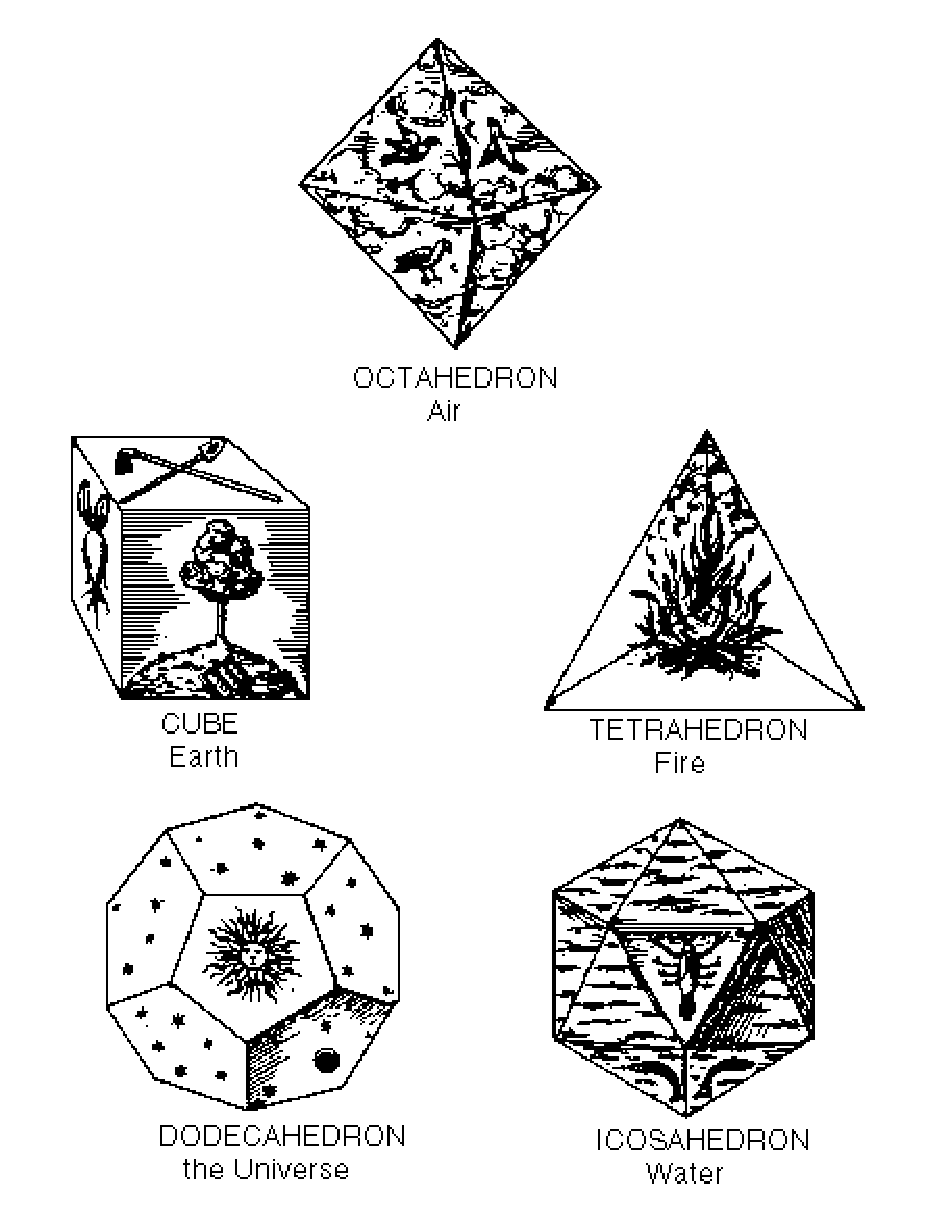
\epsfig{file=kepler.ps,width=6.1cm}
\caption{The five Platonic solids}\label{kep}

(adapted from a drawing by {\sc Kepler})
\end{center}
\end{figure}

\newpage
\noindent
{\sc Kepler} \cite{kepler} interpreted a high (resp. low) $IQ$ as wetness (resp. dryness) and 
as a justification for why the icosahedron and the tetrahedron symbolizes respectively
the water and the fire, see Fig. \ref{kep}.

\subsubsection{Fullerenes and their duals: best polyhedral approximation of a sphere?}
In \cite{g35} {\sc Goldberg} introduced, in 1935, in a slightly more general setting, the 
fullerenes (he mentions that {\sc Kirkman} \cite{kirk} found, in 1882, over $80$ 
out of the $89$ isomers of $F_{44}$). He defined, for $n\neq 18, 22$, a 
{\it medial polyhedron} with $n$ vertices as a simple polyhedron for which all 
facets are $\lfloor 6-\frac{24}{n+4}\rfloor$-gons or 
$\lfloor7-\frac{24}{n+4}\rfloor$-gons. Clearly, for 
$4\leq n\neq 18\leq 20$, the first $8$ medial polyhedra are the 8 dual convex deltahedra
and, for $20\leq n\neq 22$, medial polyhedra are the fullerenes. Therefore,
we extend the notation $F_n$ to a medial polyhedron with $n$ vertices.
Fig. \ref{goldi} reproduces those medial polyhedra, the last 9 being
$F_{20}(I_h)$, $F_{24}(D_{6d})$, $F_{26}(D_{3h})$, $F_{28}(T_d)$, $F_{28}(D_2)$,
$F_{36}(D_{3h})$, $F_{36}(D_{6h})$, $C_{60}(I_h)$ and $C_{80}(I_h)$ (called in \cite{g35}
{\it chamfered dodecahedron}). For example, $IQ(P)\simeq 0.755$, $0.906$ and $0.928$ for
$P=F_{20}(I_h)$, $C_{60}(I_h)$ and $C_{80}(I_h)$.\\

\noindent
 {\sc Goldberg} \cite{g35}
proved that the regular dodecahedron $F_{20}(I_h)$ is the best polyhedron with 12 facets and
gave the following conjecture.
\begin{conjecture}\label{cgo} {\bf [Goldberg 1935]}\\
Among polyhedra with $m$ facets, $m\neq 11,13$, a medial polyhedron 
$F_{2(m-2)}$ reaches the highest $IQ$.
\end{conjecture}
We also recall the {\sc Grace} \cite{grace} and {\sc Steiner} \cite{stein} conjectures.

\begin{conjecture}\label{cgr} {\bf [Grace 1963]}\\
Among all polyhedra with $n$ vertices lying on the unit sphere, $n\neq 18, 22$, a dual medial 
polyhedron $F^*_{n}$ reaches the highest volume.
\end{conjecture}

\begin{conjecture} {\bf [Steiner 1842]}\\
Each of the five Platonic solids reaches the highest $IQ$ among combinatorially 
equivalent polyhedra.
\end{conjecture}
The Steiner conjecture is still open for the icosahedron. If we allow any combinatorial type,
medial polyhedra  $F_{12}$ and $F_{36}(D_{6h})$ (that is, $VIII$ and $XX\!-\!2$ in terms of
Fig. \ref{goldi}) have greater $IQ$ than, respectively, the regular octahedron and icosahedron:
{\sc Goldberg} computed that $IQ(Octahedron) < IQ(F_{12})\simeq 0.628$ and
$IQ(Icosahedron) < IQ(F_{36}(D_{6h}))\simeq 0.848$.\\

The following two polyhedra given in Fig. \ref{twomissings} are almost medial and we call
them {\it quasi-medial} polyhedra with $18$ and $22$ vertices denoted by
$\tilde{F}_{18}(C_{2v})$ and $\tilde{F}_{22}(C_{2v})$. While $\tilde{F}^*_{18}(C_{2v})$ is 
the edge-coalesced icosahedron (see \cite{king}) given in Fig. \ref{coalesced},
%$\tilde{F}_{18}(C_{2v})$ itself is given page 62 in \cite{king} and
$\tilde{F}_{22}(C_{2v})$ is the one-edge truncated dodecahedron mentioned p. 274
in \cite{msbook}. This polyhedron has 10 pentagonal facets which is the maximum among all simple
polyhedra with 22 vertices. Both $\tilde{F}_{18}(C_{2v})$ and 
$\tilde{F}_{22}(C_{2v})$ and their duals are not $5$-gonal.
Another candidate to be quasi-medial polyhedron with $18$ vertices is
the one-edge truncated $F_{16}$, see \cite{msbook}.


\begin{figure}[htb]
\begin{center}
\epsfig{file=twomissings.ps,height=3.6cm}
\caption{Quasi-medial polyhedra $\tilde{F}_{18}(C_{2v})$ and
$\tilde{F}_{22}(C_{2v})$}\label{twomissings}
\end{center}
\end{figure}

\begin{figure}[phtb]
\begin{center}
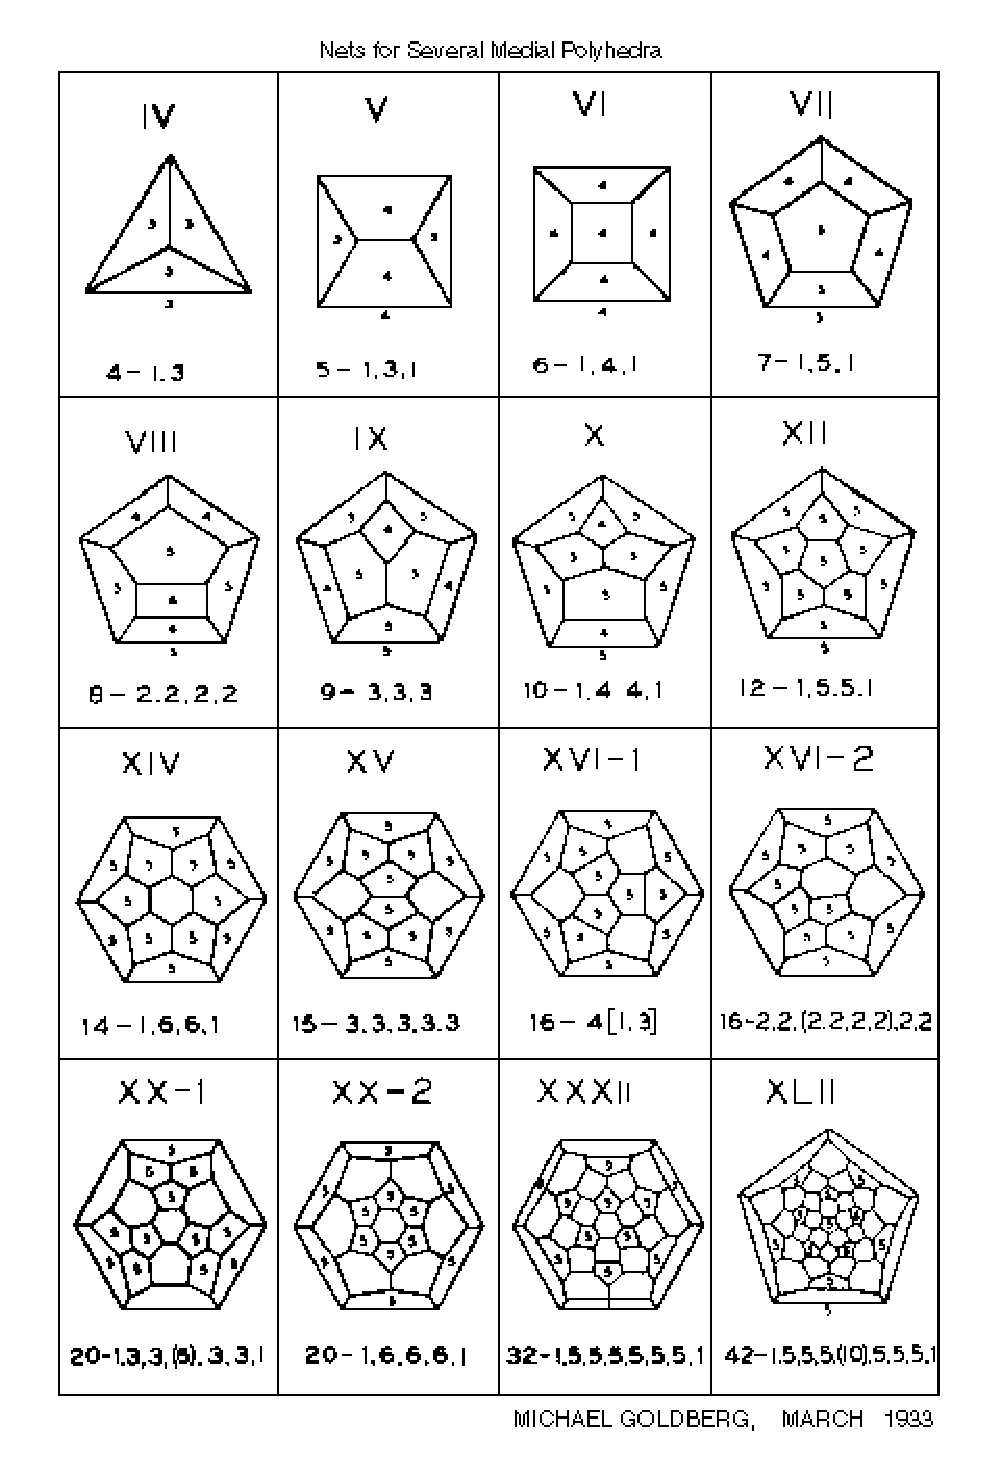
\epsfig{file=goldberg.ps,width=15.0cm}
\caption{{\sc Goldberg}'s medial polyhedra, 1933}\label{goldi}
\end{center}
\end{figure}

\newpage
\subsection{Fullerenes and other extremal problems on the sphere}
We recall the definition of the minimal energy potential $V_{n,k}$
on $n$ charges lying on the unit sphere. This notion is used, for example,
in stereo-chemistry, botany, virology, information theory and in the office
assignment problem. With $d_{pq}$ denoting the Euclidean distance between
the point charges $p$ and $q$,

%\begin{center}
%$\hspace{3cm} 
%{\displaystyle V_{n,k}= {\mbox min} \sum_{1\leq p<q\leq n}\frac{1}{d_{pq}^{k}}}.
%\hspace{3cm} (2)$
%\end{center}

\begin{displaymath}
V_{n,k}=\left\{
\begin{array}{ll}
{\displaystyle {\mbox min} \sum_{1\leq p<q\leq n}\frac{1}{d_{pq}^k}} & \mbox{for } k\geq 1\\\\
{\displaystyle {\mbox max} \sum_{1\leq p<q\leq n}\frac{1}{d_{pq}^k}} & \mbox{for } k\leq -1
\end{array}
\right.
\end{displaymath}

\noindent
{\bf Case $k=1$}.\\
This case corresponds to the Coulombic potential (the {\sc Thomson} problem).
Among the configurations minimizing $V_{n,1}$ found by {\sc Edmundson} \cite{e92},
we have the following dual fullerenes:
$F^*_4$, $F^*_6$, $F^*_{8}$, $F^*_{10}$, $F^*_{16}$, $F^*_{18}$, $F^*_{20}$,
$\tilde{F}^*_{22}$, $F^*_{24}$, $F^*_{26}$,
$F^*_{28}(T_d)$, $F^*_{30}(D_{5h})$, $C^*_{60}(I_h)$ and  $C^*_{80}(D_{5h})$.
{\sc Kuijlaar and Saff} (see \cite{ks97} and [20,21] therein) did extensive search and
indicated that for $32\leq n\leq 200$, the Voronoi domains correspond to
fullerenes with only handful of exceptions.\\

\noindent
{\bf Case $k=2$}.\\
Among the spherical Voronoi domains of the configurations minimizing $V_{n,2}$ found by
{\sc Plestenjak, Pisanski and Graovac} \cite{ppg96},
we have the following fullerenes:
$F_4$, $F_6$, $F_{8}$, $F_{10}$, $F_{14}$, $F_{16}$, $F_{18}(C_{2v})$, $F_{20}$, 
$\tilde{F}_{22}(C_{2v})$, $F_{24}$, $F_{26}$,
$F_{28}(T_d)$, $F_{30}(D_{5h})$, $F_{34}(C_2)$, $F_{36}(D_{3h})$ and $F_{40}(T_d)$.\\

\noindent
{\bf Case $k\to \infty$}.\\
This case corresponds to the {\sc Tammes} problem or densest packing by hard spheres.
For the thinnest covering (soft spheres), see {\sc Tarnai} \cite{tarnai2}, the best
known are: 
$F^*_4$, $F^*_6$, $F^*_{8}$, $F^*_{10}$, $F^*_{12}$, $F^*_{14}$, $F^*_{16}$,
$F^*_{20}$, $\tilde{F}^*_{22}(C_{2v})$, $F^*_{24}$, $F^*_{26}$,
$F^*_{28}(T_d)$, $F^*_{30}(C_{2v})$, $F^*_{32}(D_3)$, $F^*_{34}(C_{3v})$, 
$F^*_{36}(D_{2d})$, $F^*_{40}(D_{5d})$, $C^*_{60}(I_h)$, $C^*_{140}(I)$,
$C^*_{240}(I_h)$ and $C^*_{260}(I)$.\\

\noindent
{\bf Case $k=-1$}.\\
The value $\frac{V_{n,-1}}{{n\choose 2}}$ corresponds to  the maximal average distance.
For even $n$ and $d_{pq}$ the spherical metric, we have 
${\mbox max }\frac{V_{n,-1}}{{n\choose 2}}=\frac{\pi}{4}$. 

\newpage
\begin{remark}
The first 8 medial polyhedra (given in Fig. \ref{goldi}) 
can be seen as networks on the sphere, that is, 
partitions of the sphere (into $4,\dots,10$ and $12$ parts) by arcs meeting at each vertex
with equal angles of $120^o$. Together with the equipartitions of the sphere into $2$ 
and $3$ parts, they form the 10 possible partitions of this type and are the solutions
of the so-called {\sc Steiner} problem on the sphere (see \cite{heppes}).
All, except not $5$-gonal $F_{14}$ and $F_{16}$, are $\ell_1$-embeddable.
One can check (see Table 13.3.1 in \cite{grun}) that
all simple polyhedra with only 3, 4 or 5-gonal facets are those 8 items and 3
$\ell_1$-polyhedra from Figs. 7 (a), (b) and (c) of \cite{dg96}.
\end{remark}

\noindent
Small fullerenes also appear in the following forms:
\begin{itemize}
\item[$(i)$] $F_{20}$, $\tilde{F}_{22}(C_{2v})$, $F_{24}$, $F_{26}$ and $F_{28}(D_2)$
as skeletons of central soap bubbles (see Fig. 9.13 in \cite{f86})
\item[$(ii)$] $F_{20}$, $F_{24}$, $F_{26}$ and $F_{28}(T_d)$ are the only fullerenes
with {\it isolated hexagons}. In chemistry, their duals are called {\sc Frank-Kasper}
polyhedra (see \cite{fk58}).
\item[$(iii)$] The vertex sets of tetrahedral $F_{28}$, $F_{68}$, $C_{116}$ and, perhaps, 
$C_{164}$ and  $C_{188}$ appear in Table 1 of \cite{sloan} as putative best spherical 
$t$-designs with $m$ points with $(m,t)=(16,5)$, $(36,8)$, $(60,10)$, $(84,12)$ and $(96,13)$.
\item[$(iv)$] In the {\sc Mosseri-Sadoc} \cite{ms90b,msbook} models similar to the one presented in
Section \ref{4d},
small dual fullerenes such as $F^*_{20}$, $F^*_{24}$, $F^*_{26}$ and $F^*_{28}(T_d)$
appear as disclinations
(rotational defects) with respect to the vertex figure $F^*_{20}$ of the local
icosahedral order.
\item[$(v)$] Irregular $F_{20}$ with $F_{24}$ (also with $F_{28}(T_d)$, or $F_{24}$
and $F_{26}$) fills $I\hspace{-1.7mm}R^{3}$.
Those space co-fillers %$F^*_{20}$, $F^*_{24}$, $F^*_{26}$ and $F^*_{28}$
were used in pages 74, 136-139 and 659-664 in \cite{w84}
for description of clathrate crystal structures of some ice or silicate 
compounds.
Another space co-filler of $I\hspace{-1.7mm}R^{3}$ is $F_{12}$ (item VIII of Fig. \ref{goldi});
this dual of the bisdisphenoid (see Fig. \ref{rfcp} and \cite{b71,Za})
embeds into $\frac{1}{2}H_8$. We also recall that the right angled hexagonal barrel
$F_{24}$ tiles the hyperbolic space $H^3$ - it is the fundamental polyhedron of a compact 
hyperbolic manifold called the {\sc L\"obell} space which is considered also in cosmology.
The hyperbolic analogue of $F_{20}$ and $F_{\infty}$ are the following regular tilings of
the {\sc Lobachevsky} plane $H^2$: $(5,p)$  with $p>3$ by 5-gons and $(6,p)$ with $p>3$ 
by 6-gons.
Both $F_{20}$ and $F_{\infty}$ and their chamferings (defined in Section \ref{CCC})
are $\ell_1$-embeddable.
%$Cham(F_inf) = F_inf$ embeds into the cubic lattice $Z_3$).
Similarly, above two regular tilings and their chamfering are $\ell_1$-embeddable.
Moreover, any regular tiling $(n,p)$ with $\frac{1}{n}+\frac{1}{p}<\frac{1}{2}$ of the {\sc Lobachevsky} 
plane by n-gons and its chamfering embeds into the infinite dimensional cubic lattice 
$Z\hspace{-2.5mm}Z_{\infty}$ for even $n$ and into $\frac{1}{2}Z\hspace{-2.5mm}Z_{\infty}$ 
for odd $n$.
\end{itemize}


Conjectures \ref{cgo} and \ref{cgr} present the fullerenes and their duals as a kind of
best polyhedral approximation of a sphere, and the isoperimetric problem
could be the underlying issue explaining, for example,
the icosahedral structure of some virus capsids (see Section \ref{mamax}). So, this paper can
be considered as an
investigation of $\ell_1$-embeddability of supposed best polyhedral
approximation of spheres following
\cite{dg96} and \cite{ds00} which are  devoted to $\ell_1$-embedding of, respectively,  highly
regular polyhedra and infinite polyhedra (plane partitions and lattices).


%%%%%%%%%%%%%%%%%%%%%%%%%%%%%%%%% l1 full
\newpage
\section{Half-cube Embeddings of Fullerenes}
We expected the number of embeddable fullerenes to be finite and, throughout this paper,
we try to obtain the list of such fullerenes. In this Section, 
after giving some results valid for any fullerenes and 
their duals, we check the $\ell_1$-status of more than $4000$
small fullerenes and their duals. For example, the embeddability of all 
fullerenes $F_n$ for $n<60$ and preferable fullerenes $C_n$ for $n<86$ is given 
in Figs. \ref{status1} and \ref{status2}. Some infinite families
are also considered.  
The graphs were provided by {\sc G. Brinkmann} and {P. W. Fowler}
and the $\ell_1$-status was computer checked by {\sc D. Pasechnik} \cite{dima}.

\subsection{Embeddability of fullerenes and their duals}\label{sec1}
\begin{lemma}\label{cjepp}
A fullerene $F_n$ (and its dual $F^*_n$)
\begin{itemize} 
\item[(i)] either is a $\ell_1$-rigid isometric subgraph of a half-cube,
\item[(ii)] or violates a $(2k+1)$-gonal inequality for some integer $k\geq 2$.
\end{itemize}
\begin{proof} Item $(i)$ is a direct application of Lemma \ref{DeCh}. A fullerene $F_n$ being
a simple polyhedron and its dual $F^*_n$ having no vertex of valency $3$, both do not contain
$K_4$ and therefore are $\ell_1$-rigid (and isometric subgraph of a half-cube
by the implications given at the end of Section \ref{kointro}) when $\ell_1$-embeddable.
If $F_n$ or $F^*_n$ is not embeddable: recall, as remarked in~\cite{dg93},
that a hypermetric but not $\ell_1$-embeddable
graph has diameter 2 or 3. Then, since $F^*_{20}$ is known to be an $\ell_1$-polyhedron and since any fullerene 
(and its dual except $F^*_{20}$) has diameter at least $4$, $(ii)$ follows.
\end{proof}
\end{lemma}

While there exist 5-gonal but not 7-gonal polyhedra, for example the snub 
square antiprism (see \cite{b71,Za}), we could not find any such fullerene. 
This and Lemma \ref{cjepp} lead us to the following conjecture:

\begin{conjecture}\label{violat}
 A fullerene $F_n$ (and its dual $F^*_n$)
\begin{itemize}
\item[(i)] either is $\ell_1$-rigid,
\item[(ii)] or violates a 5-gonal inequality.
\end{itemize}
\end{conjecture}

\subsection{Embeddings of small fullerenes}\label{sec2}
\begin{figure}[htb]
\begin{center}
\begin{tabular}{|c|c|c|} \hline
Fullerene & $\ell_1$-embeddability of $F_n$ & $\ell_1$-embeddability of $F^*_n$ \\ \hline \hline
$F_{20}(I_h)$ & $\rightarrow\frac{1}{2}H_{10}$ & $\rightarrow\frac{1}{2}H_{6}$\\ \hline
$F_{26}(D_{3h})$ & $\rightarrow\frac{1}{2}H_{12}$ & not 5-gonal \\ \hline
$F_{28}(T_d)$ & not 5-gonal & $\rightarrow\frac{1}{2}H_{7}$ \\ \hline
$F_{36}(D_{6h})$ & not 5-gonal & $\rightarrow\frac{1}{2}H_{8}$ \\ \hline
$F_{44}(T)$ & $\rightarrow\frac{1}{2}H_{16}$ & not 5-gonal \\ \hline
\end{tabular}
 
\caption{Embeddability of small fullerenes}\label{status1}
({\em Out of all $7916$ $F_n$ and $F^*_n$ with $n< 60$, 
only 6 are $\ell_1$-embeddable})
\end{center}

\begin{center}
\begin{tabular}{|c|c|c|} \hline
Fullerene & $\ell_1$-embeddability of $F_n$ & $\ell_1$-embeddability of $F^*_n$ \\ \hline \hline
$C_{60}(I_h)$ & not 5-gonal & $\rightarrow\frac{1}{2}H_{10}$ \\ \hline
$C_{80}(I_h)$ & $\rightarrow\frac{1}{2}H_{22}$ & not 5-gonal \\ \hline
\end{tabular}

\caption{Embeddability of small preferable fullerenes}\label{status2}
({\em Out of all 102 $C_n$ and $C^*_n$ with $n< 86$, 
only 2  %$C_{80}(I_h)$ and $C^*_{60}(I_h)$ 
are $\ell_1$-embeddable})
\end{center}
\end{figure}

Out of more than $4000$ fullerenes 
$F_n$ and their duals for $n<60$, and all preferable fullerenes 
$C_n$ and their duals for $n<86$, only $4$ fullerenes,
$F_{20}(I_h)$, $F_{26}(D_{3h})$, $F_{44}(T)$, and $C_{80}(I_h)$, 
and only $4$ dual fullerenes,
$F^*_{20}(I_h)$, $F^*_{28}(T_d)$, $F^*_{36}(D_{6h})$ and $C^*_{60}(I_h)$,
turn out to be $\ell_1$-embeddable (see Figs. \ref{status1} and \ref{status2}). 
The embeddings  
are given in detail in Figs. 
\ref{embeddingofF20}, 
\ref{embeddingofF26}, 
\ref{embeddingofF44} and 
\ref{embeddingofdualC60} where a vertex of $\frac{1}{2}H_m$ is labeled 
by the set $S\subset\{1,2,\dots,m\}$ of its nonzero coordinates  ($\bar{S}$ 
denotes the complement of $S$). For example, the lower vertex $v$ of the central 
pentagon of Fig. \ref{embeddingofF20} is labeled by $\{4,5\}$, that is, 
$v=\{0,0,0,1,1,0,0,0,0,0\}$ of $\frac{1}{2}H_{10}$.
In Fig. \ref{embeddingofC80}, the edges are labeled by the symmetric difference
between sets of nonzero coordinates of corresponding vertices of $\frac{1}{2}H_{22}$.
The embeddings of $F_{20}(I_h)$ and its dual are trivial (see, for example, \cite{dl94}) 
and the embeddings of $F_{26}(D_{3h})$ and $F^*_{28}(T_d)$ are given in \cite{dg96}.

\begin{figure}[htb]
\begin{center}
\epsfig{file=embeddingofF20.ps,width=5.0cm}
\caption{Embedding of $F_{20}(I_h)$ into $\frac{1}{2}H_{10}$}\label{embeddingofF20}
\end{center}
\end{figure}

\begin{figure}[hbt]
\begin{center}
\epsfig{file=embeddingofF26.ps,width=5.0cm}
\caption{Embedding of $F_{26}(D_{3h})$ into $\frac{1}{2}H_{12}$}\label{embeddingofF26}
\end{center}
\end{figure}

\begin{figure}[hbt]
\begin{center}
\epsfig{file=embeddingofF44.ps,width=7.6cm}
\caption{Embedding of $F_{44}(T)$ into $\frac{1}{2}H_{16}$}\label{embeddingofF44}
\end{center}
\end{figure}

\begin{figure}[hbtp]
\begin{center}
\epsfig{file=embeddingofC80.ps,width=9.7cm}
\caption{Embedding of $C_{80}(I_h)$ into $\frac{1}{2}H_{22}$}\label{embeddingofC80}
\end{center}
\end{figure}

\clearpage

\begin{figure}[phtb]
\begin{center}
\epsfig{file=Embedding_Dual.ps,width=13.0cm}
\caption{Embedding of $F^*_{20}(I_h)$, $F^*_{28}(T_d)$, $F_{36}^*(D_{6h})$ and $C_{60}^*(I_h)$ into, respectively, 
$\frac{1}{2}H_{6}$, 
$\frac{1}{2}H_{7}$,
$\frac{1}{2}H_{8}$
and $\frac{1}{2}H_{10}$}\label{embeddingofdualC60}
\end{center}
\end{figure}

\clearpage

\subsection{Infinite families of non $\ell_1$-fullerenes}
In this section we present two families of non $\ell_1$-fullerenes based on a construction
analogous to {\sc Fowler} \cite{atlas} carbon cylinder construction which gives preferable fullerenes. 
Starting
from a fullerene $F_n$ that we can separate into two {\it hemispheres} by cutting $5$ edges 
(resp. $6$), we insert between those hemispheres a layer of $5$ hexagons (resp. $6$). The obtained
fullerene has $n+10$ vertices (resp. $n+12$) and is called a {\it $1$-layered $F_n$}. By inserting
$i$ layers, we get the $i$-layered $F_n$. 
For example, cutting anywhere $F_{20}$
and inserting $i$ layers, we get the $i$-layered dodecahedron defined
as $F_{10(i+2)}(D_{5h})$ for odd $i$ and $F_{10(i+2)}(D_{5d})$ for even $i$ (see Fig. \ref{F40}).
Starting with 
$F_{24}(D_{6d})$ and inserting $i$-layers of $6$ hexagons between two hemispheres made of
$5$ pentagons surrounding a hexagon, we get the $i$-layered $F_{24}(D_{6d})$: $F_{12(i+2)}(D_{6h})$
for odd $i$ and $F_{12(i+2)}(D_{6d})$ for even $i$, see Fig. \ref{F40}.
Those two families were introduced in Table 5 of \cite{fow87} as dihedral 
fullerenes with two caps.

\begin{figure}[htb]
\begin{center}
\epsfig{file=F40.ps,height=5.0cm}
\caption{$F_{36}(D_{6h})=1$-layered $F_{24}(D_{6d})$ and $F_{40}(D_{5d})=2$-layered
dodecahedron}\label{F40}
\end{center}
\end{figure}
\begin{proposition}\label{strained} For any integer $i\geq 1$:
\begin{itemize} 
\item[(i)] The $i$-layered fullerene (and its dual) $F_{10(i+2)}(D_{5h}\mbox{ or }D_{5d})$  
is not $\ell_1$-embeddable, and
\item[(ii)] the $i$-layered fullerene (and its dual except for $i\!=\!1$) $F_{12(i+2)}(D_{6h}\mbox{ or }D_{6d})$
is not $\ell_1$-embeddable.
\end{itemize}
\begin{proof}
To prove that the above fullerenes are not $\ell_1$-embeddable, we simply exhibit a non 5-gonal
configuration contained in their skeletons. The coefficients $b_i$ of the violated 
5-gonal inequality (see Eq. $(1)$ of Section \ref{intro})
are, respectively, $0$ for a black vertex, $-1$ for a square one, and $1$ for a white circle.

\newpage
\begin{center}
\epsfig{file=5gonalF10n.ps,width=9.0cm}

The non 5-gonal configurations of $i$-layered $F_{10(i+2)}$ for $i=1$ and for $i\geq 2$. 
\end{center}

\begin{center}
\epsfig{file=5gonalF12n.ps,width=9.0cm}

The non 5-gonal configurations of $i$-layered $F_{12(i+1)}$ for $i=1$ and for $i\geq 2$.
\end{center}

\begin{center}
\epsfig{file=dualF30.ps,width=9.0cm}

The non 5-gonal configurations of dual $i$-layered $F^*_{12(i+1)}$ and $F^*_{10(i+1)}$
for $i\geq 3$.
\end{center}
\end{proof}
\end{proposition}

Item $(i)$ of Proposition \ref{strained} was given in \cite{dg96} where $i$-layered
dodecahedra were called {\it strained fullerenes} and introduced as duals of 2-capped towers
of $(i+1)$ pentagonal antiprisms. Those fullerenes can be seen as somehow 
opposite to preferable fullerenes $C_n$, that is, with many pentagons sharing a common
edge. See also Propositions \ref{champ} and \ref{many} where many other families of non
$\ell_1$-fullerenes are given.

\clearpage
%%%%%%%%%%%%%%%%%%%%%%%%%%%%%%%%%%%%%%% Icosahedral
%\newpage
\section{Icosahedral Fullerenes}
To determine if $\ell_1$-embeddability is more likely to occur for fullerenes with 
large symmetry, we focus on {\em icosahedral fullerenes}, that is,
fullerenes with either the extended icosahedral group 
$I_h$ of order 120 or the {\it proper} icosahedral group $I$ (=$A_5$). % containing only rotations. 

\subsection{Icosahedral fullerenes}\label{tria}
Any icosahedral fullerene $F_n(I_h)$ and $F_n(I)$ comes by folding of
triangular net and satisfies $n=20T$ with {\it triangulation number}
$T=a^2+ab+b^2$ for positive integers
$(a,b)$, see \cite{c71,g37}. All icosahedral fullerenes being preferable except
$F_{20}(I_h)$, we denote them $C_{20T}(I_h)$ or $C_{20T}(I)$ by abuse of notation.
Moreover, $n=60i$ if $(a-b)$ is divisible by $3$, and $n=60i+20$
otherwise. The symmetry group of an icosahedral fullerene is $I_h$ for $ab=0$ or $a=b$, 
and $I$ otherwise. For example, the first icosahedral fullerene $F_{20}(I_h)$
corresponds to $(a,b)=(1,0)$; the $C_{60}(I_h)$ corresponds
to $(a,b)=(1,1)$; and the {\em chamfered dodecahedron} (see {\sc Goldberg} 
\cite{g35}) $C_{80}(I_h)$ corresponds to $(a,b)=(2,0)$ (see Figs. \ref{c60} 
and \ref{c80}, or item XLII of Fig. \ref{goldi}). 
In other words, an icosahedral fullerene is the (a,b)-generalized 
leapfrog of a dodecahedron (see {\sc Sah} \cite{s94}) or the $\{5+,3\}_{a,b}$
(see {\sc Coxeter} \cite{c71}). 

\begin{figure}[hb]
\begin{center}
\epsfig{file=C60.ps,width=5cm}
\caption{The $C_{60}(I_h)$ or $(1,1)$-dodecahedron}\label{c60}
\end{center}
\begin{center}
\epsfig{file=C80.ps,width=5cm}
\caption{Chamfered dodecahedron $C_{80}(I_h)$}\label{c80}
{\it $(2,0)$-dodecahedron}
\end{center}
\end{figure}

\subsection{Dual icosahedral fullerenes}
Call {\em icosadeltahedron} the duals - $C^*_{20T}(I_h)$ or $C^*_{20T}(I)$ - of an
icosahedral fullerene. Those icosadeltahedra were introduced by {\sc Goldberg} \cite{g37} in 1937
and (independently) by {\sc Caspar and Klug} \cite{ck62} in 1962 as capsids
(protein coats) of some viruses. The first icosadeltahedron is the icosahedron
$F^*_{20}(I_h)$; and, for $(a,b)=(1,1)$, we have the dual buckminsterfullerene $C^*_{60}(I_h)$
which is also the pentakis dodecahedron denoted $\{3,5+\}_{1,1}$ by {\sc Coxeter}.
In Fig. \ref{escher}, $C^*_{60}(I_h)$ can be seen represented as omnicapped dodecahedron
in {\em Gravitation} of {\sc Escher}, which can also be seen as a small stellated 
dodecahedron with pentagram faces. 

\begin{figure}[hb]
\begin{center}
\epsfig{file=dualC80.ps,width=6.7cm} 

$C^*_{60}(I_h)$
\end{center}
\begin{center}
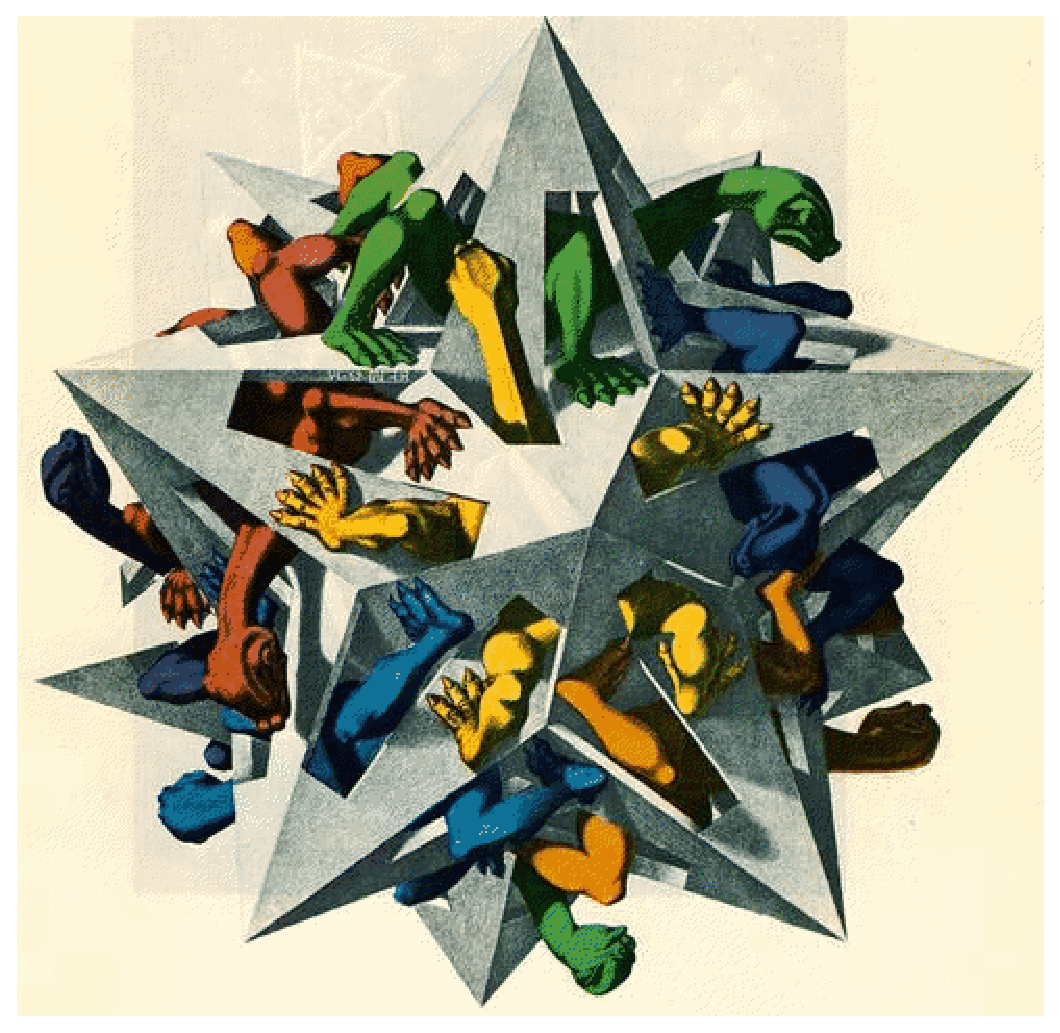
\epsfig{file=escher.ps,width=5cm}
\caption{{\sc Gravitation (1952)}}\label{escher}
{\it omnicapped dodecahedron}
\end{center}
\end{figure}

\begin{remark} 
Another interesting family of dual fullerenes is the hypothetical 
boron cages (for example, see \cite{bl77}). 
The first one, $B_{12}=F^*_{20}(I_h)$, 
is known experimentally: $[B_{12}H_{12}]^{2-}$.
Next cases are:
$B_{14}=F^*_{24}(D_{6d})$,
$B_{15}=F^*_{26}(D_{3h})$,
$B_{16}=F^*_{28}(T_d)$,
$B_{17}=$ all three $F^*_{30}$,
$B_{18}=$ three  $F^*_{32}$,
$B_{19}=$ three $F^*_{34}$,
$B_{20}=$ three $F^*_{36}$,
$B_{21}=$ three $F^*_{38}$,
$B_{22}=$ three $F^*_{40}$ including $F^*_{40}(T_d)$,
$B_{23}=$ three $F^*_{42}$,
$B_{24}=$ six $F^*_{44}$ including $F^*_{44}(T)$.
Next cases with tetrahedral or higher symmetry are 
$B_{28}=F^*_{52}(T)$, 
$B_{32}=C^*_{60}(I_h)$ and
$B_{92}=C^*_{180}(I_h)$. 
The last two are fairly stable in terms of eigenvalues of the H\"uckel 
Hamiltonian (see \cite{chin}). 
Both dual quasi-medial polyhedra $\tilde{F}^*_{18}(C_{2v})$ and $\tilde{F}^*_{22}(C_{2v})$ - see
Fig. \ref{twomissings} - are also putative boron cages for $B_{11}$
and $B_{13}$.
\end{remark}


\begin{figure}[htbp]
\begin{center}
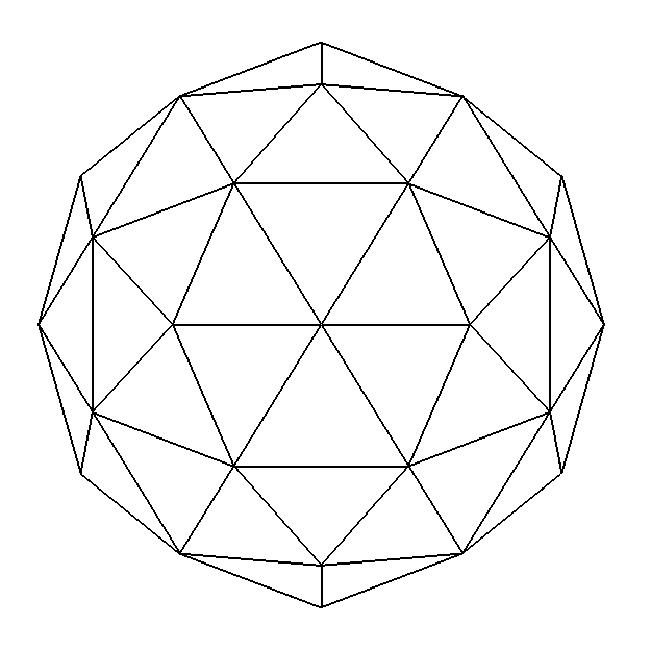
\epsfig{file=heche2dode.ps,width=6cm}

$C^*_{80}(I_h)$
\end{center}
\begin{center}
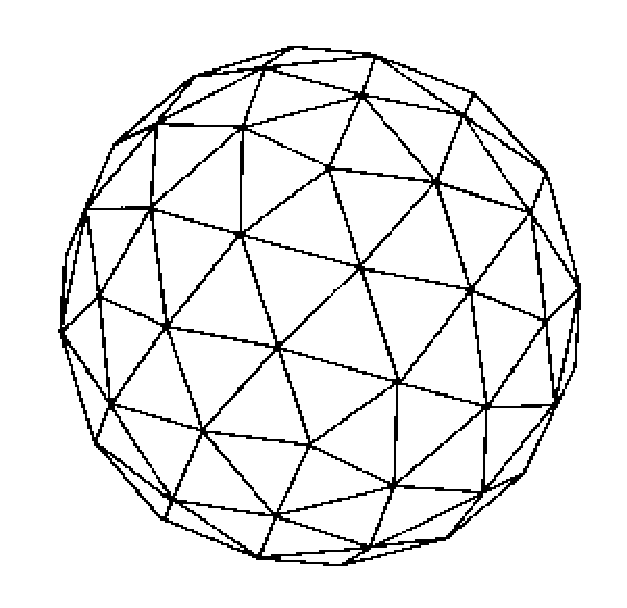
\epsfig{file=cox140.ps,width=7cm}

$C^*_{140}(I)$
\end{center}
\begin{center}
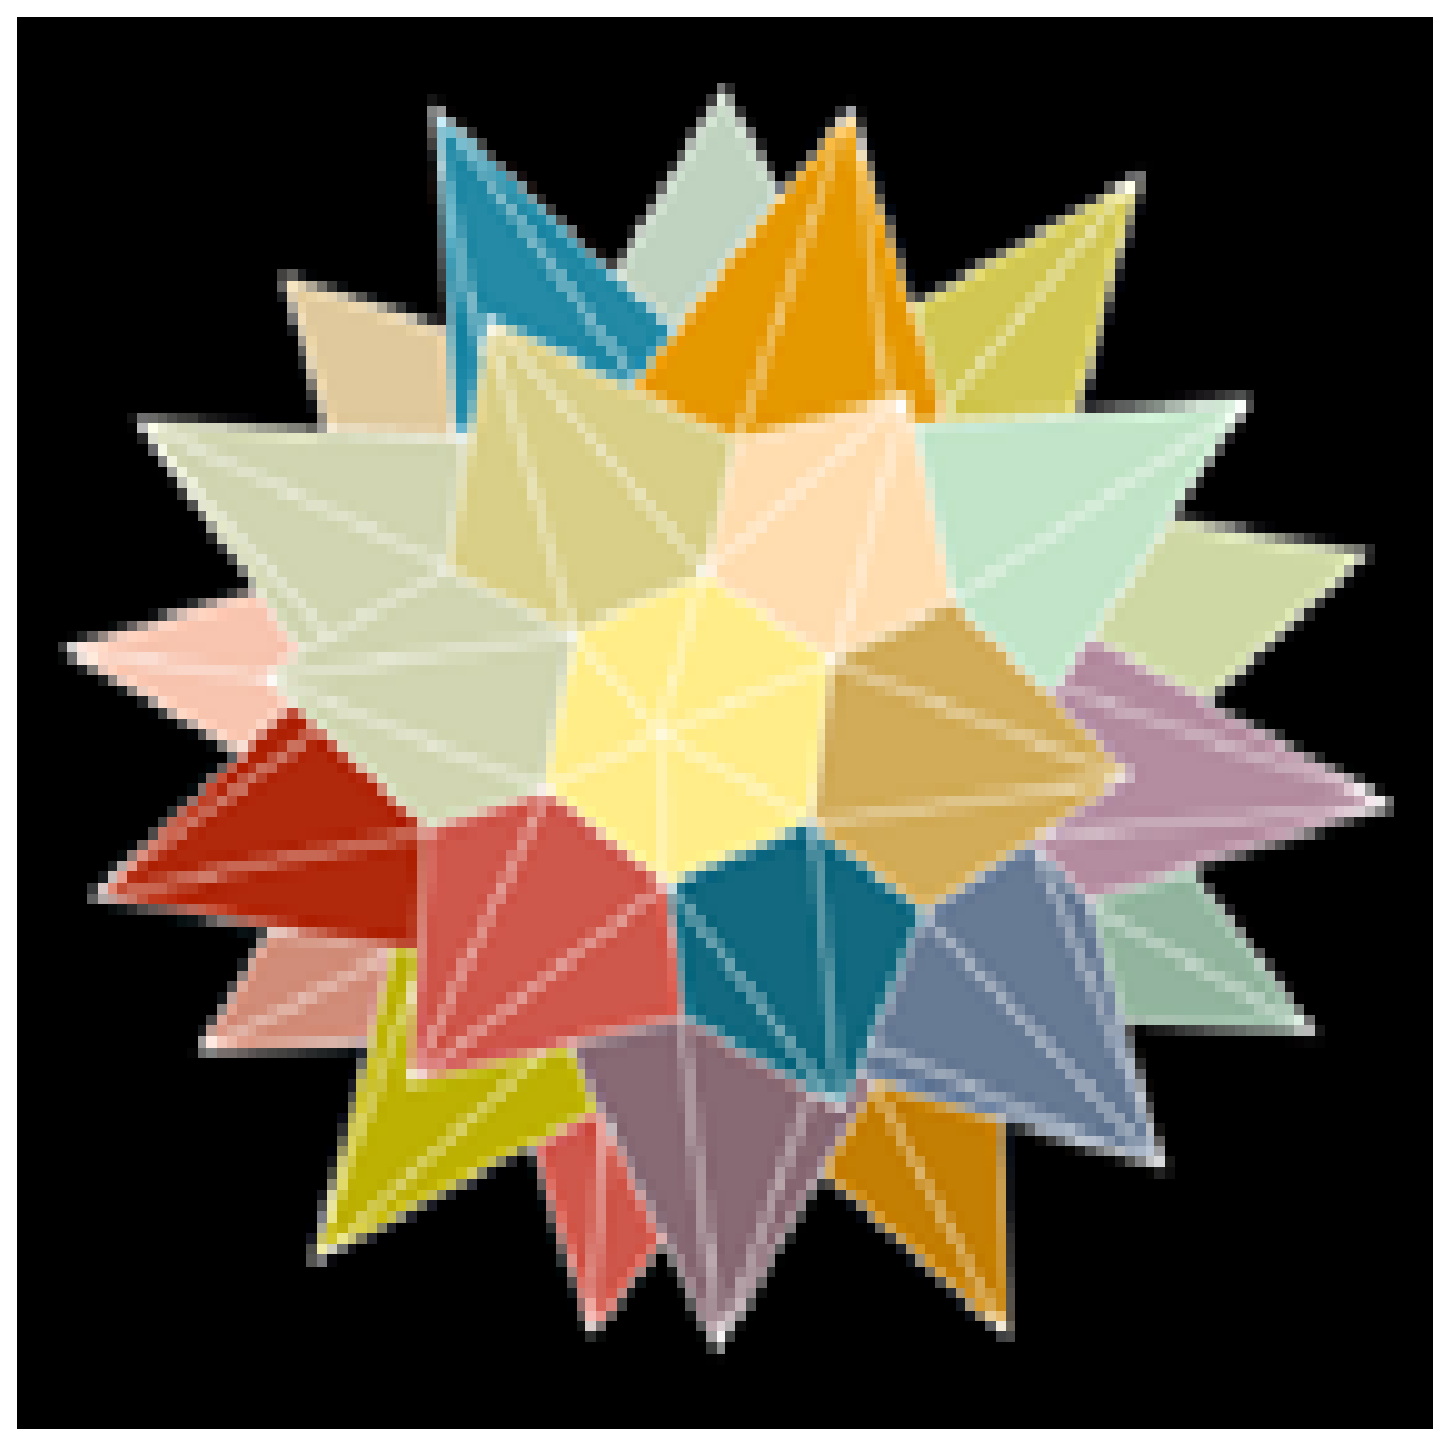
\epsfig{file=etoile1.ps,width=6cm}

$C^*_{180}(I_h)$ as omnicapped buckminsterfullerene

\caption{Three icosadeltahedra}
\end{center}
\end{figure}

\clearpage
\newpage
\subsection{Geodesic domes and virus capsids}\label{mamax}
In this Section - which follows an approach similar to {\sc Tarnai} \cite{tarnai} -
we present icosahedral fullerenes and their
duals, the icosadeltahedra, which occur as geodesic domes
and as capsids of viruses. In Figs. \ref{domes} and \ref{virus}, the
pair of integers $(a,b)$ characterizing the triangulation number $T$
is given for each dome or virus (see Section \ref{tria}). {\it Laevo}
(resp. {\it dextro}) denotes the icosahedral fullerene $C_{20T}(I)$
with $a>b>0$ (resp. with $b>a>0$). 

\subsubsection{Geodesic domes}
Since {\sc Fuller}'s patent in 1954, numerous geodesic domes has been built. Some of the
most famous, including the Iena test planetarium of 1922, are given in Fig. \ref{domes}.
In architecture, the value $f=a+b$ is called the {\it frequency}; icosahedral fullerenes
with $ab=0$ are of type 1, same with $a=b$ are of type $2$, and remaining laevo and dextro
fullerenes $C_{20T}(I)$ are of type $3$ (types $1$ and $2$ correspond to 
{\it alternate}
and {\it triacon} in {\sc Fuller} terms). Remark that almost all domes of Fig. \ref{domes}
are of type $1$, few are of type $2$ and only one is of type $3$ (and laevo).
\begin{figure}[htbp]
\begin{center}
\begin{tabular}{|c|c|c|} \hline
$(a,b)$ & Fullerene & Geodesic dome \\ \hline \hline
$(1,0)$ & $F^*_{20}(I_h)$ & {\it One of Salvatore Dali houses} \\ \hline
$(1,1)$ & $C^*_{60}(I_h)$ & {\it Arctic Institute, Baffin Island} \\ \hline
$(2,0)$ & $C^*_{80}(I_h)$ & {\it Playground toy, Kjarvalstadir, Iceland} \\ \hline
$(3,0)$ & $C^*_{180}(I_h)$ & {\it Bachelor officers quarters, US Air Force, Korea} \\ \hline
$(2,2)$ & $C^*_{240}(I_h)$ & {\it U.S.S. Leyte } \\ \hline
$(3,1)$ & $C_{260}(I)_{laevo}$ & {\it Statue in Gagarin city, Russia} \\ \hline
$(4,0)$ & $C^*_{320}(I_h)$ & {\it Geodesic Sphere, Mt. Washington, New Hampshire} \\ \hline
$(5,0)$ & $C^*_{500}(I_h)$ & {\it US pavilion, Trade Fair 1956, Kabul, Afghanistan} \\ \hline
$(3,3)$ & $C_{540}(I_h)$ & {\it Hafnarfj\"ordur dome, Iceland} \\ \hline
$(6,0)$ & $C^*_{720}(I_h)$ & {\it Radome, Arctic DEW} \\ \hline
$(6,0)$ & $C_{720}(I_h)$ & {\it Bath at a golf course, Tokyo} \\ \hline
$(4,4)$ & $C^*_{960}(I_h)$ & {\it Sky Eye radio telescope} \\ \hline
$(8,0)$ & $C^*_{1280}(I_h)$ & {\it German pavilion, Osaka Expo} and {\it Accra dome, Ghana} \\ \hline
$(6,6)$ & $C_{2160}(I_h)$ & {\it Children camp pavilion, Vyshod, Russia}  \\ \hline
$(12,0)$ & $C_{2880}(I_h)$ & {\it Children camp pavilion, Kirov, Russia} \\ \hline
$(8,8)$ & $C^*_{3840}(I_h)$ & {\it Spaceship Earth, Epcot center, Florida} and {\it Lawrence, Long Island} \\ \hline
$(16,0)$ & $C^*_{5120}(I_h)$ & {\it Test planetarium, Iena 1922} and {\it US pavilion, Expo '67, Montreal} \\ \hline
$(16,0)$ & $C_{5120}(I_h)$ & {\it Internal layer of US pavilion, Expo '67, Montreal} \\ \hline
$(18,0)$ & $C^*_{6480}(I_h)$ & {\it G\'eode du Mus\'ee des Sciences, La Villette, Paris} \\ \hline
$(18,18)$ & $C_{19440}(I_h)$ & {\it Union Tank Car Co., Baton Rouge, Louisiana} \\ \hline
\end{tabular}
\caption{Icosahedral fullerenes as geodesic domes}\label{domes}
\end{center}
\end{figure}
\begin{figure}[htbp]
\begin{center}
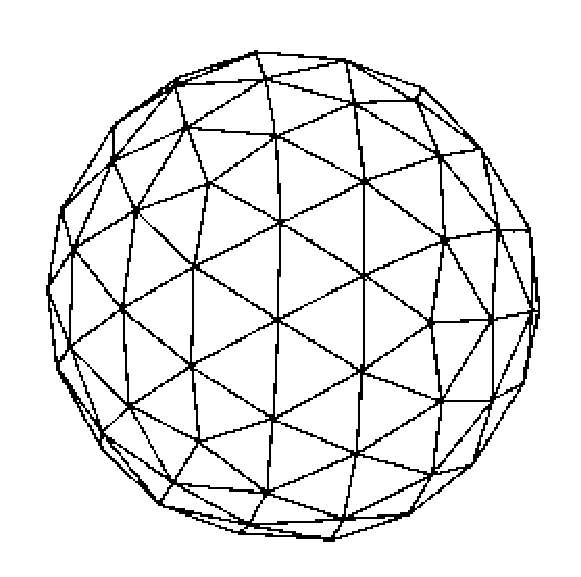
\epsfig{file=cox180.ps,width=6cm}
\caption{Icosadeltahedron $C^*_{180}(I_h)$}\label{korea}
{\it Bachelor officers quarters, US Air Force, Korea}
\end{center}
\end{figure}

\newpage
\subsubsection{Icosahedral virus capsids}
A pair of icosadeltahedra of type $(a,b)$ and $(b,a)$ with $a>b>0$ are 
mirror images of each other (or {\it enantiomorpheous}) 
- for example, $C^*_{140}(I)_{laevo}$
and $C^*_{140}(I)_{dextro}$. 
%The frequency $f=a+b$ and the triangulation number $T=a^2+ab+b^2$
%are also used are in architecture. 
The icosahedral structure of HIV-1 and iridovirus are proved, but the $(6,3)$ value
for the HIV-1 is still to be confirmed, and the $(10,4)$ value for the iridovirus is also, even if less
commonly, considered. Remark that the majority of viruses of Fig. \ref{virus} are with symmetry $I_h$
and especially of type $(a,0)$. And among the remaining with symmetry $I$, only one is dextro
(see \cite{ddub} for a presentation of icosahedral viruses).
The discovery 
that the majority of human virulent viruses are icosahedral 
recalls Plato's belief that an excess of water - which element
was supposed to be the icosahedron - is one of the main reasons for sickness.

\begin{figure}[htbp]
\begin{center}
\begin{tabular}{|c|c|c|} \hline
$(a,b)$ & Fullerene & Icosahedral virus capsid \\ \hline \hline
$(1,0)$ & $F^*_{20}(I_h)$ & {\it Gemini virus} \\ \hline
$(1,1)$ & $C^*_{60}(I_h)$ & {\it Turnip yellow mosaic virus} \\ \hline
$(2,0)$ & $C^*_{80}(I_h)$ & {\it Bacteriophage {\em $\Phi R$}} \\ \hline
$(2,1)$ & $C^*_{140}(I)_{laevo}$ & {\it Rabbit papilloma virus} \\ \hline
$(1,2)$ & $C^*_{140}(I)_{dextro}$ & {\it Human wart virus} \\ \hline
%$(3,0)$ & $C^*_{180}(I_h)$ & {\it Outer shell of reovirus} \\ \hline
$(3,1)$ & $C_{260}(I)_{laevo}$ & {\it Rotavirus} \\ \hline
$(4,0)$ & $C^*_{320}(I_h)$ & {\it Herpes virus, varicella} \\ \hline
$(5,0)$ & $C^*_{500}(I_h)$ & {\it Infectious canine hepatitis virus, adenovirus} \\ \hline
$(6,0)$ & $C^*_{720}(I_h)$ & {\it HTLV-1}\\ \hline
$(6,3)$ & $C^*_{1260}(I)_{laevo}$ & {\it HIV-1}, {\small usually admitted value value}\\ \hline
$(7,7)$ & $C^*_{2940}(I_h)$ & {\it Iridovirus}; {\small also considered value $(10,4)$}\\ \hline
\end{tabular}
\caption{Icosahedral fullerenes as virus capsids}\label{virus}
\end{center}
\end{figure}
\begin{figure}[htbp]
\begin{center}
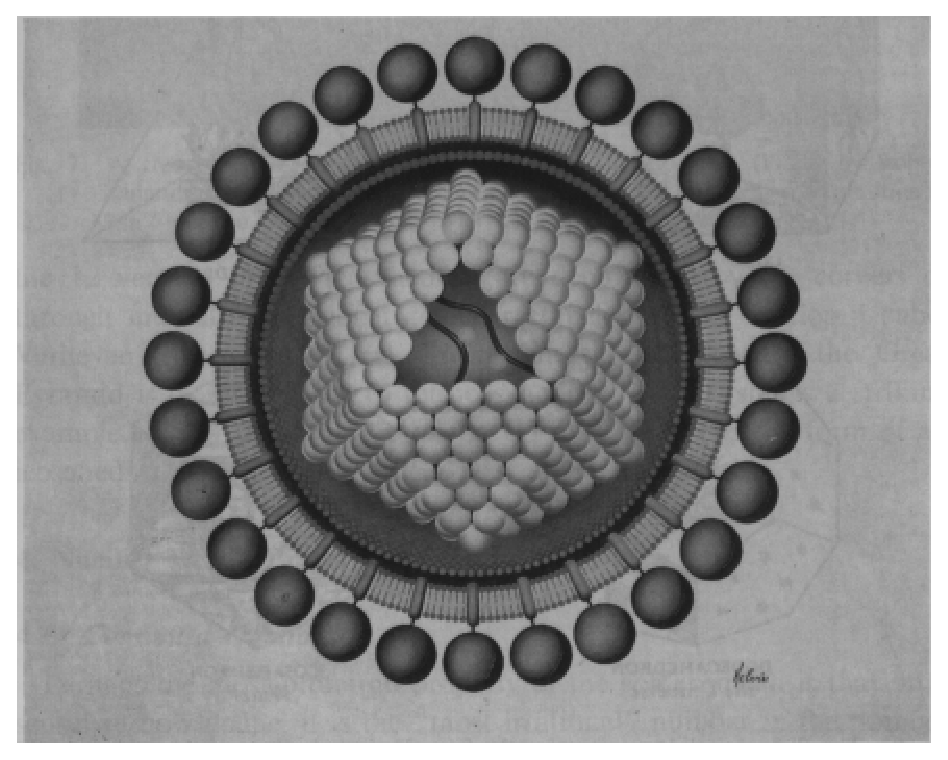
\epsfig{file=aids.ps,width=7.5cm}
\caption{The icosahedral structure $C^*_{720}(I_h)$ of the HTLV-1}\label{aids}
%{\it From "The First Human Retrovirus^^ ^^ ,  by Robert C. Gallo. Illustration by George\\ 
% V. Kelvin, Science Graphics. $\copyright$ 1986 by Scientific American. Inc.
%}
\end{center}
\end{figure}

\begin{remark}
There are exactly 8 combinatorially distinct {\it simple
quasi-crystal forms}, that is, polyhedra with symmetry group 
$I_h$ or $I$ transitive on the facets (see for example \cite{ge92}).
Namely, the icosahedron and dodecahedron embed into $\frac{1}{2}H_6$
and $\frac{1}{2}H_{10}$, respectively, and, among the six icosahedral
Catalan polyhedra, the triacontahedron (= dual icosidodecahedron), the dual truncated 
icosahedron, and the dual truncated dodecahedron embed 
into $H_6$, $\frac{1}{2}H_{10}$ and $\frac{1}{2}H_{26}$, respectively.
The other three Catalan polyhedra, the dual rhombic icosidodecahedron, the dual truncated
icosidodecahedron and the snub dodecahedron, are not $5$-gonal.
\end{remark}

\begin{figure}[hb]
\begin{center}
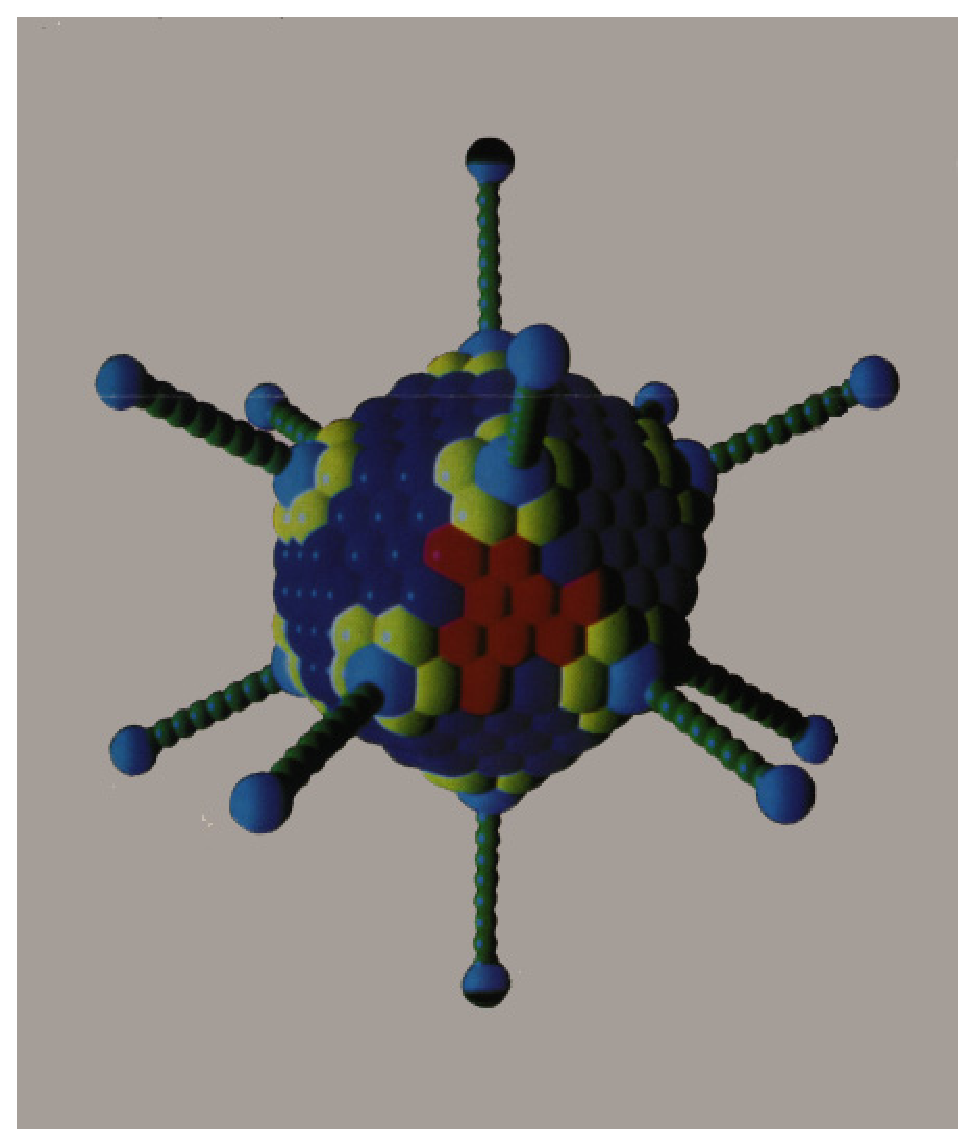
\epsfig{file=virus.ps,width=7.0cm}
\caption{Computer simulated adenovirus $C^*_{500}(I_h)$ with its spikes}\label{adenovirus}

\end{center}
\end{figure}

%%%%%%%%%%%%%%%%%%%%%%
\newpage
\subsection{Embedding of icosahedral fullerenes}
The first icosahedral fullerenes with $ab\neq 0$ and $a\neq b$, that is, with 
symmetry group $I$, are laevo and dextro $C_{140}(I)$
with either $(a,b)=(2,1)$ or $(1,2)$. These fullerenes (and their duals) are
non $\ell_1$-embeddable as well as $C _{60}(I_h)$ 
which is a $(a,a)$-fullerene with $a=1$. We focus on
icosahedral fullerenes with $b=0$, that is, $C_{20a^2}(I_h)$.

\subsubsection{The $(a,0)$-dodecahedron}
Since the icosahedral fullerene $C_{20a^2}(I_h)$ comes as a $(a,0)$-generalized 
leapfrog of the dodecahedron, we call it the {\it 
$(a,0)$-dodecahedron}.  
For example, the $(1,0)$-dodecahedron is the dodecahedron itself, the 
$(2,0)$-dodecahedron is Goldberg chamfered dodecahedron $C_{80}(I_h)$ given in
Fig. \ref{c80} (or item XLII of Fig. \ref{goldi}) and the $(3,0)$-dodecahedron 
is $C_{180}(I_h)$, represented in 
Fig. \ref{edo}, taken from {\it Sanpo-Kiriko-Shu} by {\sc Yasuaki Aida} 
(1747-1817) (see {\sc Miyazaki} \cite{m92}).

\begin{figure}[hbt]
\begin{center}
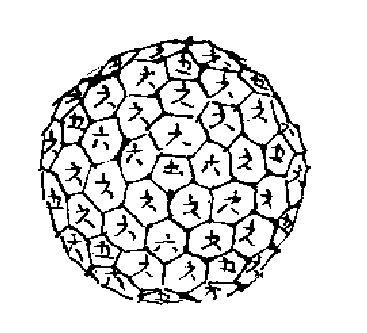
\epsfig{file=sphere1.ps,width=6cm}
\caption{The $(3,0)$-dodecahedron $C_{180}(I_h)$}\label{edo}

{\it from Sanpo-Kiriko-Shu, Edo era}
\end{center}
\end{figure}


\begin{proposition}\label{champ} 
Besides the dodecahedron, the icosahedron and the chamfered dodecahedron,
the $(a,0)$-dodecahedron $C_{20a^2}(I_h)$ and its dual are not $\ell_1$-embeddable. 
\begin{proof}
First, we recall the combinatorial structure of $C_{20a^2}(I_h)$.
Identifying any  pentagon with the ring $R_0$, we can see $C_{20a^2}(I_h)$
being made up of $3a+1$ rings of facets. For example, $R_1$ is made of the 5
hexagons surrounding $R_0$ and $R_{3a}$ is the pentagon opposite to $R_0$.
See also the
figure below where the $10$ hexagons of the ring $R_3$ of $C_{80}(I_h)$ are in grey.

\begin{center}
\epsfig{file=proof.ps,width=3.5cm}
\end{center}

More generally, the rings $R_i$ and $R_{3a-i}$ are congruent for $0\leq i\leq 3a$.
The rings containing pentagons are $R_0$ and $R_{3a}$ with 1 pentagons and no hexagon
and $R_{a}$ and $R_{2a}$ with $5$ pentagons and $5(a-1)$ hexagons. The remaining
rings $R_i$ (without any pentagon) contain $5a$ hexagons for $a\leq i \leq 2a$
and $5i$ hexagons for $0<i<a$ or $2a<i<3a$. For $1\leq i\leq 3a$,
denote by $C_i$ the set of edges separating two adjacent rings $R_{i-1}$ and $R_i$,
and call a hexagon of $R_i$ {\em simple} (resp. {\em meridian}) with 2 (resp. 3)
edges in $C_i$ and 2 (resp. 1) edges in $C_{i-1}$; $R_0$ and $R_{3a}$ being seen
as north and south poles of $C_{20a^2}(I_h)$. Clearly,
$R_i$ contains exactly 5 meridian hexagons
for $0<i<a$ or $2a<i<3a$ and only simple ones for $a\leq i \leq 2a$. For example,
each pentagon
of $R_a$ is connected to $R_0$ by a chain of $(a-1)$ meridian hexagons
and to two other pentagons of $R_a$ by a chain of $(a-1)$ simple hexagons of $R_a$.
By contracting those chains to an edge, the rings $R_0,R_1\dots R_a$ collapse to
the half-dodecahedron and, by doing the same for all pentagons, $C_{20a^2}(I_h)$
collapses to the dodecahedron.

%Call {\em opposite} two edges of a hexagon without a common vertex. The
%transitive closure of the relation {\em to be opposite} on the edges of
%$C_{20a^2}(I_h)$ gives an equivalence relation $O$ which generates $30$ classes
%of equivalent edges
%containing exactly 2 edges belonging to pentagons and $6(a-1)$ classes containing
%edges belonging to hexagons only. 
%Directly applying the algorithm given
%in \cite{ds96}, we can now label the edges of $C_{20a^2}(I_h)$ with the same
%pair $(i,j)$ for equivalent edges. The embedding of the dodecahedron into
%$\frac{1}{2}H_{10}$ gives a labeling of the $30$ classes containing edges of
%pentagons by pairs $(i,j)$ with $1\leq i<j\leq 10$. Then, we label the $6(a-1)$
%remaining classes by $6(a-1)$ disjoint pairs $k,l$ with $11\leq k<l\leq 10+12(a-1)$
%- those classes being exactly the $6(a-1)$ hexagonal convex cuts separating a pair
%of opposite pentagons. In other words, $C_{20a^2}(I_h)$ embeds into
%$\frac{1}{2}H_{2(6a-1)}$.

To prove that $C^*_{20a^2}(I_h)$ is $\ell_1$-embeddable only for $a=1$,
we first recall some definitions. The skeleton of $C_{20a^2}(I_h)$ being of
valency 3 and planar, a path entering a vertex $v$ can exit it either by the
right edge or the left one. A path or circuit for which the edges can be alternatively
labeled as left or right are called {\em alternating}. The skeleton of a polyhedron $P$
is uniquely covered by the family of all alternating circuits where each edge belongs
to at most $2$ circuits. If each circuit is not self-intersecting, that is, if
each edge belongs to exactly $2$ circuits, we call the family of alternating circuits
{\em complete}.
Then, if all alternating circuits of a complete family correspond to the convex cuts of the
skeleton of $P^*$, this family gives an $\ell_1$-embedding of $P^*$. Namely, indexing all
the circuits, each edge of $P^*$ is labeled by the 2 indices of the circuits containing it.
We first check if $C^*_{20a^2}(I_h)$ has a complete family of alternating circuits. Clearly,
the circuits $C_i$ separating rings $R_{i-1}$ and $R_i$ form alternating circuits
for $a< i \leq 2a$; each $C_i$ containing $10a$ edges. Since we have 6 pairs of
opposite pentagons, by changing the basic pentagon $R_0$ we get $6a$ circuits. In the
figure below,
the dotted line is the circuit $C'_4$ with $R_0$ moved to $R'_0$.
\begin{center}
\epsfig{file=proof2.ps,width=5.5cm}
\end{center}
By construction, each edge of $C_{20a^2}(I_h)$ belongs to at most 2 circuits. Now, since each of 
those
$6a$ circuits contain $10a$ edges, the family contains at least $30a^2$ edges, that is, exactly
the number of edges of $C_{20a^2}(I_h)$ - which implies that the family is complete. But, even if
$C_{20a^2}(I_h)$ has a complete family, $C^*_{20a^2}(I_h)$ is not $\ell_1$-embeddable because those
alternating circuits of $C_{20a^2}(I_h)$ do not give convex cuts of $C^*_{20a^2}(I_h)$ for $a>1$. 

Now we prove that $C_{20a^2}(I_h)$ is not embeddable for $a>2$ by showing 
that its unique possible labeling do not give convex cuts. For $a>2$, we have at least 
2 rings $R_k$, $a<k<2a$ which consist only of hexagons.
These rings are separated by circuits $C_k$, $a+1<k<2a$ and the edges of the ring
$R_k$ connecting vertices of the circuits $C_k$ and $C_{k+1}$ have the
same labels. Hence, these edges determine cuts that we denote also by $R_k$.
Actually the cuts $R_k$ are not convex. Suppose that $R_k$ are convex and
consider two adjacent rings $R_{k-1}$ and $R_k$ separated by the circuit 
$C_k$. Recall that if cuts ($X_1,Y_1$) and ($X_2,Y_2$) are convex, then the
intersections $X_1$ with $X_2$, $Y_1$ with $Y_2$ and $X_i$ with $Y_j$ are
also convex.
Let $R_k=(X_k,Y_k)$ $a<k<2a$ and $X_k$ contains the pentagon $R_0$.
Then the intersection $Y_{k-1}$ with $X_k$ consists only of the vertices of $C_k$.
This means that any two points of $C_k$ are connected by a unique shortest
path (going in $C_k$) if these points are not antipodal - while for antipodal
points there are two shortest paths.
Now, consider another system of rings $R'_k$ where $R'_0$ is a pentagon
distinct from $R_0$ and $R_{3a}$. This system determines a circuit $C'_k$
separating two convex cuts $R'_{k-1}$ and $R'_k$. This circuit $C'_k$ has a
non-empty intersection with $C_k$ consisting of two edges $x$ and $y$.
These two edges are opposite in both the circuits $C_k$ and $C'_k$ that are
even. Consider one endpoint of $x$ and one endpoint of $y$. These endpoints
are connected by at least two distinct shortest paths going in $C_k$ and
$C'_k$. This contradiction proves that the cuts $R_k$ cannot be convex.
Moreover $C_{20a^2}(I_h)$ is not 5-gonal. Actually, consider two hexagons 
$h_k$ and $h'_k$ belonging to $R_k\cap R'_k$. 
These hexagons contain the edges $x$ and $y$ with, say, $x in h_k$, and
$y\in h'_k$. Take an endpoint $v$ of $y$ and two opposite edges of $h_k$
distinct from $x$. The endpoints of these opposite edges and $v$ form
a non 5-gonal configuration
- which completes the proof. 

\end{proof}
\end{proposition}

\begin{remark}
The fullerenes $F_{56}(T_d)$ and $C_{140}(I_h)$ also have a complete family
of circuits giving nonconvex cuts in their duals which, therefore,
are not $\ell_1$-embeddable.
Actually, all known $\ell_1$-fullerenes are somehow exeptional.
Besides the dodecahedron $F_{20}(I_h)$ which is exceptionnal in many ways, 
$F_{26}(D_{3h})$ and $F_{80}(I_h)$ have induced subgraphs which are 
not 5-gonal but both are not isometric, $F_{26}(D_{3h})$ and $F_{44}(T)$ 
admit nonconvex 
alternating cuts, that is, some - only one for $F_{44}(T)$ - convex cuts 
defining their embedding are not alternating.
\end{remark}

%\newpage
\subsubsection{Chamfered dodecahedron}\label{CCC}
We now consider special case of $(a,0)$-dodecahedron where $a=2^t$ for an 
integer $t$. Since $C_{80}(I_h)$ was named the {\it chamfered dodecahedron} by 
{\sc Goldberg} in \cite{g35}, we call {\it $t$-chamfered dodecahedron} the 
$(2^t,0)$-dodecahedron $C_{20\cdot2^{2t}}(I_h)$. Clearly, the $0$-chamfered 
dodecahedron is the dodecahedron itself, the $1$-chamfered dodecahedron
is the chamfered dodecahedron and the $2$ and $4$-chamfered dodecahedra 
are, respectively, $C_{320}(I_h)$ and $C_{5120}(I_h)$ - the dual of Mt. Washington 
and of Iena planetarium presented in Fig. \ref{domes}.  
Those $t$-chamfered dodecahedra are the result
of the ($t$-times) edge truncation illustrated by Fig. \ref{chamfering}, which was
also given in
\cite{fow87} as the {\it quadrupling transformation} for fullerenes.
The chamfering - also used by {\sc Gr\"unbaum} \cite{grun} p. 263 -
as well as the leapfrog operation were introduced in 1891 by  {\sc Eberhard} in \cite{eber91} 
p. 180 as, respectively, $\Pi_2$ and $\Pi_1$ constructions. 

\begin{figure}[hbtp]
\begin{center}
\epsfig{file=chamfering.ps,width=7.0cm}
\caption{The chamfering edge truncation}\label{chamfering}
\end{center}
\end{figure}

\clearpage
\newpage
For any polyhedron $P$, denote $Cham_t(P)$ the $t$-times chamfered $P$.
Each vertex $v$ of $P$ will valency $k_v$ with create $k_v$ new vertices in $Cham_1(P)$
and each edge of $P$ will create a hexagon. So, the $f$-vector of the chamfering
of a polyhedron $P$ with 
constant vertex incidence $k$ is $f(Cham_1(P))=((k+1)f_0(P),k\:f_0(P)+2 f_1(P), f_1(P) + f_2(P))$
and the $p$-vector is preserved except $p_6(Cham_1(P))=p_6(P)+f_1(P)$.
For a fullerene, the chamfering corresponds to a (2,0)-leapfrog transform and 
we have $Cham_1(F_n(S_g))=C_{4n}(S_g)$
where $S_g$ is the symmetry group of $F_n$.
We also recall in Fig. \ref{loeb} the well-known edge truncation
given in Chap. 10 of {\sc Loeb} \cite{loeb}.
 
\begin{figure}[htbp]
\begin{center}
\epsfig{file=loeb.ps,width=7.0cm}
\caption{Usual edge truncation}\label{loeb}
\end{center}
\end{figure}

\begin{proposition}\label{nonl1}$\:$\\
With the definition of alternating circuits given in the proof of Proposition \ref{champ},
two necessary conditions for the $\ell_1$-embeddability of the $t$-chamfered fullerene $(2^t,0)$-$F_n$ are:
\begin{itemize}
\item[(i)] $F_n$ is $\ell_1$-embeddable and
\item[(ii)] the family of alternating circuits of $F_n$ is complete.
\end{itemize} 
\begin{proof}
By induction, it is enough to prove it for the $1$-chamfering. Let denote
by $E(F_n)$ the set of edges of $F_n$ and by $Cham(F_n)$ the chamfering
of $F_n$. We have $E(Cham(F_n))=E_1(Cham(F_n))\cup E_2(Cham(F_n))$
where there is a one-to-one correspondence between pairs of parallel {\it old}
edges of new hexagons of $E_1(Cham(F_n))$  and the edges $E(F_n)$, and where the {\it new}
edges $E_2(Cham(F_n))$ are the edges of $Cham(F_n)$ shared by the new
hexagons of $Cham(F_n)$. Now, assume that $F_n$ is $\ell_1$-embeddable.
Using the same terminology as for the proof of Proposition \ref{champ},
the $\ell_1$-embeddability into $\frac{1}{2}H_m$ of $F_n$ means that we can 
label its edges by pairs: $(i,j)$ $1\leq i<j\leq m$ such that equivalent 
edges are labeled
by the same pair (see, for example, Fig. \ref{embeddingofC80}).
Then, since by construction the chamfering preserves the equivalence
relation, the $\ell_1$-embeddability of $Cham(F_n)$ implies the
$\ell_1$-embeddability of $F_n$ (same labeling for $E_1(Cham(F_n))$
and for $E(F_n)$). To prove $(ii)$, we notice that edges of $E_2(Cham(F_n))$
are partitioned into equivalence classes not intersecting with 
equivalence classes of $E_1(Cham(F_n))$, moreover those equivalence
classes of $E_2(Cham(F_n))$ are in one-to-one correspondence with
the alternating circuits of $F_n$. Now, if $Cham(F_n)$ is 
$\ell_1$-embeddable, the equivalence classes of $E_2(Cham(F_n))$
are precisely the convex cuts of $Cham(F_n)$ and the corresponding
alternating circuits of $F_n$ form the complete family of alternating
circuits. Which completes the proof.
\end{proof}
\end{proposition}

\begin{proposition}\label{many}
Applying item $(i)$ of Proposition \ref{nonl1}, 
for any integer $\geq t$, the following families 
of fullerenes are not $\ell_1$-embeddable:
$C_{60\cdot 2^{2t}}(I_h)$, 
$C_{140\cdot 2^{2t}}(I)$, 
$C_{28\cdot 2^{2t}}(T_d)$, 
$C_{56\cdot 2^{2t}}(T_d)$ and  
$C_{76\cdot 2^{2t}}(T_d)$. 
By item $(ii)$, for any integer $\geq t$,
the $t$-chamfered $F_{26}(D_{3h})=C_{26\cdot 2^{2t}}(D_{3h})$ is not $\ell_1$-embeddable.
\end{proposition}

\begin{remark}
Taking the pentakis (capping of all pentagons) of
dodecahedron, icosidodecahedron $(7)$, snub dodecahedron $(18)$, pentagonal orthobirotunda $(54)$ (also called anti-icosi\-dode\-ca\-he\-dron)
gyroelongated pentagonal birotunda $(68)$, we obtain $C^*_{60}(I_h)$, $C^*_{80}(I_h)$,
$C^*_{140}(I)$, $C^*_{80}(D_{5h})$ (i.e. the dual twisted $Cham(F_{20}(I_h))$) 
and a $C^*_{100}$.
The 3 regular-faced polyhedra numbers $(7)$, $(54)$ and $(68)$ (see \cite{b71})
come from the pentagonal rotunda $M_{9}$; precisely, $(7)=M_9+\overline{M}_9$,
 $(54)=2\:M_9$ and $(68)=M_9+Antiprism_{10}+M_9$. Those 3 polyhedra are not 5-gonal, 
the snub dodecahedron is $\ell_1$-rigid embeddable into $\frac{1}{2}H_{15}$;
$C^*_{80}(I_h)$, $C^*_{140}(I)$, $C^*_{80}(D_{5h})$ and $C^*_{100}$ are not 5-gonal.
\end{remark}

\subsubsection{Edge truncations}
The Loeb edge truncation of the 5 Platonic solids gives 3 Archimedean
zonohedra. Namely, by this edge truncation the tetrahedron becomes the truncated
octahedron, both octahedron and cube become
the truncated cuboctahedron and both
icosahedron and dodecahedron become the truncated icosidodecahedron.
For the same 5 Platonic solids,
the chamfered tetrahedron is the dual 4-capped octahedron (the capped facets
being pairwise non-adjacent), 
the chamfered icosahedron (resp. dodecahedron) is the dual triakis (resp. pentakis) 
icosidodecahedron and the chamfered cube (resp. octahedron) is the dual tetrakis (resp. triakis) 
cuboctahedron. Actually, any zonohedron being
embeddable into a cube, the chamfered cube, which is a simple zonohedron,
embeds into $H_{7}$; its generators are 
$e_1, e_2, e_3, (e_1\pm e_2)$ and $(e_1\pm e_3)$. 
On the other hand, the chamfering of the $Prism_6$ and the rhombic dodecahedron,
which are both zonohedra, gives polyhedra which are neither zonohedra nor $\ell_1$-embeddable.
The chamfered cube provides the following nice link between the dodecahedron
and the rhombic dodecahedron (dually, the transition between the icosahedron and the 
cuboctahedron is known in chemistry, see~\cite{w84} p.146). The chamfered cube 
is, on the one hand, partially (on the six $4$-valent vertices) the vertex-truncation of the 
rhombic dodecahedron and, on the other hand, is partially (on the six edges linked
pairwise by no less than two edges) the Loeb edge-truncation of the 
dodecahedron. 

\begin{remark}
The proof of Proposition \ref{nonl1} never using that $F_n$ is a fullerene - 
it holds for the chamfering of any polyhedron. The tetrahedron
is an example of polyhedron for which the chamfering is not $\ell_1$-embeddable
while satisfying the conditions of Proposition
\ref{nonl1}. 
\end{remark}

\begin{proposition}
Among the Platonic solids, their chamferings and the duals of their chamferings,
only the tetrahedron, the octahedron, the icosahedron, the cube and its chamfering, the dodecahedron
and its chamfering and dual chamfered tetrahedron are $\ell_1$-embeddable.
Moreover, they embed into $\frac{1}{2}H_{2\delta}$ where $\delta$ denotes the diameter 
of the polyhedron except the tetrahedron - which is $\frac{1}{2}H_{3}$ - and the dual chamfered tetrahedron which embeds into
$\frac{1}{2}H_{8}$ while its diameter is $3$. 
Recall that all known embeddable fullerenes (and all embeddable dual fullerenes
except $F^*_{28}(T_d)\to\frac{1}{2}H_{7}$ while $\delta(F^*_{28}(T_d))=4$)
embed into $\frac{1}{2}H_{2\delta}$.
The $(a,0)$-cube and its dual are not $\ell_1$-embeddable for $a\geq 3$. 
\end{proposition}

\newpage
\subsection{Quasi-embeddings of $C_{60}$ and $F^*_{60}(C_s)_r$}
{\bf Quasi-$C_{60}$}.\\
Even if $C_{60}$ is not $\ell_1$-embeddable, we still can {\em quasi}-embed it 
into $\frac{1}{2}H_{20}$ in the
following sense. We consider a relaxation of the notion of $\ell_1$-embedding
which allows us to find the
$\ell_1$-metric somehow {\em closest} to the $C_{60}$. We say that a metric $d$ 
is {\em $t$-embeddable} if there is
an $\ell_1$-embeddable metric $d'$ such that $d'_{i,j}=\:min(d_{i,j},t)$ .
This notion was introduced in \cite{ds96} where it was shown  that the
polynomial algorithm given there for the recognition
of $\ell_1$-graph can be extended to the recognition of $t$-embeddable graphs.
In particular, a unique $3$-embedding into $\frac{1}{2}H_{20}$ of $C_{60}$,
called {\em quasi}-$C_{60}$, which is also a $7$-embedding, is given there.
Moreover, quasi-$C_{60}$ is an $\ell_1$-rigid (but not graphic) metric.
There are at least two $2$-embeddings of $C_{60}$. Actually any simple 
polyhedron with $m$ facets admits a $2$-embedding into $\frac{1}{2}H_m$
where each vertex is associated to the 3 facets containing it; therefore
any $F_{60}$ is 2-embeddable into $\frac{1}{2}H_{32}$. The Fig. \ref{7embeddingofC60} illustrates the $7$-embedding of $C_{60}$.
The construction is the following: to each of the $20$ hexagons we can associate a coordinate of
$I\hspace{-1.7mm}R^{20}$. Then a vertex $v$ (for example the white atom of Fig.
\ref{7embeddingofC60})
is mapped to the vertex $\phi(v)$ of the odd half-cube $\frac{1}{2}\overline{H}_{20}$  whose
non zero coordinates correspond to the $7$ hexagons of $C_{60}$
containing a vertex with distance to $v$ is
less than $3$ (the $7$ grey hexagons of Fig. \ref{7embeddingofC60}). This
give us a $7$-embedding of $C_{60}$ into the odd half-cube
$\frac{1}{2}\overline{H}_{20}$, and by adding modulo $2$ any $\phi(v)$ to all
the $60$ vertices of quasi-$C_{60}$ we get a $7$-embedding into $\frac{1}{2}H_{20}$.
All distances of length $8$ and $9$ in $C_{60}$ became $7$ in quasi-$C_{60}$
(recall that $C_{60}$ has diameter $9$). It could be interesting to compare the
automorphism group of quasi-$C_{60}$ (i.e. all the permutations of the $20$ coordinates indexed by
the $20$ hexagons
of $C_{60}$ which preserve quasi-$C_{60}$) with the one of $C_{60}$, which is the 
icosahedral group $A_5$.
The Fig. \ref{spiral} illustrates one automorphism of quasi-$C_{60}$ we found: the reversing of the
spiral Hamiltonian path on the $20$ hexagons of $C_{60}$.

\begin{figure}[htb]
\begin{center}
\epsfig{file=7embeddingofC60.ps,height=5.0cm}
\caption{Embedding up do distance $7$ of $C_{60}(I_h)$ into 
$\frac{1}{2}H_{20}$}\label{7embeddingofC60} 
\end{center}
\end{figure}

\begin{figure}[htb]
\begin{center}
\epsfig{file=spiral.ps,height=5.0cm}
\caption{The spiral Hamiltonian automorphism of quasi-$C_{60}$}\label{spiral}
\end{center}
\end{figure}

\newpage
\noindent
{\bf Quasi-$F^*_{60}(C_s)_r$}.\\
The dual of $F_{60}(C_s)_r$, considered in Section \ref{sec2},
admits a $4$-embedding into $\frac{1}{2}H_{10}$.
More precisely, $F^*_{60}(C_s)_r$ has diameter $5$ and all distances are preserved
except between $4$ opposite pentagons:
$(\overline{38},48)$,
$(\overline{1378},1478)$,
$(\overline{45},35)$
and
$(\overline{2459},2359)$.
Instead of $5$, those distances became $4$ in $\frac{1}{2}H_{10}$. See Fig. \ref{4embeddingofF60},
where the vertices of
$F^*_{60}(C_s)_r$ are labeled as facets of $F_{60}(C_s)_r$
and where a non 5-gonal configuration of $F_{60}(C_s)_r$ is given.
\begin{figure}[htb]
\begin{center}
\epsfig{file=quasiright.ps,height=8.0cm}
\caption{The $4$-embedding $F^*_{60}(C_s)_r$ into $\frac{1}{2}H_{10}$
and a non 5-gonal configuration of $F_{60}(C_s)_r$}\label{4embeddingofF60}
\end{center}
\end{figure}

\newpage
\section{Other Chemically Relevant Polyhedra and Fullerene Analogues}
\subsection{Coordination polyhedra, metallopolyhedra and Bravais lattices}
\subsubsection{Coordination polyhedra and metallopolyhedra}
According to {\sc Wells} \cite{w84}, the chemical crystal structure is usually described by
$a)$ the {\em coordination polyhedron}:
the convex hull of anions forming the group of nearest neighbours of each metal ion;
or $b)$ the {\em domain of atom} (Voronoi-Dirichlet polyhedron).
Coordination polyhedra are arrangements of nearest neighbours in crystals, molecules and ions.
More precisely, as defined by {\sc Frank and Kasper} in \cite{fk58}, a {\em coordination 
polyhedron}
is the convex hull of the mirror images of the center of a Voronoi-Dirichlet domain in each of its
faces. Remark that the coordination polyhedron is, in general, 
not dual to the Voronoi-Dirichlet
domain, and different from the contact polytope of sphere packing.
For example, while the Voronoi-Dirichlet 
polyhedron of a point of the lattice $A_3^*$ 
(body-centered cubic lattice) is the truncated octahedron, its coordination polyhedron is the rhombic
dodecahedron. 
In addition to some frequent coordination polyhedra, the $\ell_1$-status of some
metallopolyhedra (convex hull of atoms of metallic cluster) or metal and
oxygen polyhedra (see \cite{ddmp93,king,thim,w84}) % p. 76-78 
are given in Fig. \ref{rfcp}.
The names and the number (as regular-faced polyhedra) are taken
from the list of such 112 polyhedra given in \cite{b71,Za}. For example, see Fig. \ref{twisted}
where the embedding of the rhombicuboctahedron $(13)$ and the non $5$-gonality of 
the twisted one $(57)$ are given.

\begin{figure}[htb]
\begin{center}
\epsfig{file=twisted.ps,width=10.5cm}
\caption{The rhombicuboctahedron embeds into $\frac{1}{2}H_{10}$, the snub cube
into $\frac{1}{2}H_{9}$ and the twisted rhombicuboctahedron is not $5$-gonal}\label{twisted}
\end{center}
\end{figure}

\begin{figure}[pthb]
\begin{center}
\begin{tabular}{|c|c|c|} \hline
Polyhedron ($n^o$ as regular-faced) & $\ell_1$-embeddability & Example \\ \hline \hline
$Tetrahedron$ (1) & $\rightarrow\frac{1}{2}H_{3}$ & $Rh_4(CO)_{12}$ \\ \hline
$Octahedron$ (2) & $\rightarrow\frac{1}{2}H_{4}$ & $[Os_6(CO_{18})]^{2-}$ \\ \hline
$Cube$ (3) & $\rightarrow H_{3}$ & $CsCl$ \\ \hline
$Icosahedron$ (4) & $\rightarrow\frac{1}{2}H_{6}$ & [$Mo_{12}O_{30}(CeO_{12})]^{8-}$ \\ \hline
$Cuboctahedron$ (6) & not 5-gonal & $[Mo_{12}O_{36}(SiO_4)]^{4-}$ \\ \hline
%$Cuboctahedron$ (6) & not 5-gonal & $[Mo_{6}O_{19}]^{2-}$ \\ \hline
{\em Truncated tetrahedron} (8) & not 5-gonal & $[Mo_{12}(HOAsO_3)_4O_{34}]^{4-}$ \\ \hline
$Rhombicuboctahedron$ (13) & $\rightarrow\frac{1}{2}H_{10}$ & $[V_{18}O_{42}(SO_4)]^{8-}$ \\ \hline
{\em Triangular prism} (19) & $\rightarrow\frac{1}{2}H_{5}$ & $[Rh_6C(CO)_{15}]^{2-}$ \\ \hline
{\em Square antiprism} (20) & $\rightarrow\frac{1}{2}H_{5}$ & $[Co_8C(CO)_{18}]^{2-}$ \\ \hline
{\em Square pyramid} (21) & $\rightarrow\frac{1}{2}H_{4}$ & $Fe_5C(CO)_{15}$ \\ \hline
{\em Triangular cupola} (23) & not 5-gonal & $[W_{9}O_{30}(PO_4)]^{9-}$ \\ \hline
{\em Gyroelongated square pyramid} (30) & extreme hypermetric & $[Co_9Si(CO)_{21}]^{2-}$ \\ \hline
{\em Triangular bipyramid} (32) & $\rightarrow\frac{1}{2}H_{4}$ & $Os_5(CO)_{16}$ \\ \hline
{\em Pentagonal bipyramid} (33) & not 5-gonal  & $K_3ZrF_7$ \\ \hline
{\em Elongated square bipyramid} (35) & $\rightarrow\frac{1}{2}H_{6}$ & $[W_{10}O_{32}]^{4-}$ \\ \hline
{\em Gyroelongated square bipyramid} (37) & extreme hypermetric & $[V_{10}O_{26}]^{4-}$ \\ \hline
{\em Triangular orthobicupola} (47) & not 5-gonal & $[W_{12}O_{36}(SiO_4)]^{4-}$ \\ \hline
%{\em Triangular orthobicupola} (47) & not 5-gonal & $[H_2Rh_{13}(CO)_{24}]^{3-}$ \\ \hline
{\em Square gyrobicupola} (49) & not 5-gonal & $[V_{10}O_{26}]^{4-}$ \\ \hline
{\em Elongated triangular bicupola} (55) & not 5-gonal & $\alpha$-$[W_{18}P_2O_{62}]^{6-}$ \\ \hline
{\em Elongated triangular gyrobicupola} (56) & not 5-gonal & $\beta$-$[W_{18}P_2O_{62}]^{6-}$ \\ \hline
{\em Twisted rhombicuboctahedron} (57) & not 5-gonal & $[H_4V_{18}O_{42}(Br)]^{9-}$ \\ \hline
{\em Elongated pentagonal bicupola} (58) & not 5-gonal & $[W_{30}P_5O_{110}(Na)]^{14-}$ \\ \hline
{\em Augmented triangular prism} (69) & $\rightarrow\frac{1}{2}H_{5}$  & $Na_5Zr_2F_{13}$ \\ \hline
{\em Biaugmented triangular prism} (70) & $\rightarrow\frac{1}{2}H_{5}$  & $N_2H_6(ZrF_6)$ \\ \hline
{\em Triaugmented triangular prism} (71) & extreme hypermetric  & $Eu(OH)_3$ \\ \hline
{\it Bisdisphenoid} (104) & not 5-gonal  & $K_4ZrF_8$ \\ \hline
$Octahedron+Pyramid_3$ & $\rightarrow\frac{1}{2}H_{5}$ & $[Ru_7(CO_{16}]^{3-}$ \\ \hline
$Octahedron+2\:Pyramid_3$ & $\rightarrow\frac{1}{2}H_{6}$ & $[Os_8(CO_{22}]^{2-}$ \\ \hline
$Tetrahedron+2\:Pyramid_3$ & $\rightarrow\frac{1}{2}H_{5}$ & $[Os_6(CO_{18}]^{2-}$ \\ \hline
{\it Edge-coalesced icosahedron} & extreme hypermetric & $[B_{11}H_{11}]^{2-}$ \\ \hline
\end{tabular}
\caption{Embeddability of some of the most frequent chemical polyhedra}\label{rfcp}
\end{center}
\end{figure}

\newpage
\begin{remark}\label{bidi}
The regular-faced polyhedra from Fig. \ref{rfcp} with numbers 1, 2, 4, 32, 33, 37, 71 and
104 are the 8 convex deltahedra with regular facets and with $n$ vertices
$4\leq n\leq 12$, $n\neq 11$.
Those deltahedra are dual of the first 8 medial polyhedra $F_n$ given in Fig. \ref{goldi} 
with $n=4,8,20,6,10,16,14$ and $12$.
%(with corresponding numbers: $1,32,2,33,104,71,37$ and $4$).
The edge-coalesced icosahedron is a
deltahedron with 11 vertices but with irregular facets. By deleting one of the curved edges
of Fig. \ref{coalesced} we obtain the regular-faced augmented sphenocorona $(107)$ with one
facet a square. Both are {\it extreme hypermetric} (see \cite{dg93,dl96}) and, together with the 1-capped $Antiprism_5$, 
can be seen as quasi-deltahedra with 11 vertices.

\begin{figure}[bht]
\begin{center}
\epsfig{file=coalesed.ps,width=2.6cm}
\caption{The edge-coalesced icosahedron}\label{coalesced}
\end{center}
\end{figure}
\end{remark}

\begin{remark}
The last three $\ell_1$-embeddable polyhedra of Fig. \ref{rfcp} are capped or 
2-capped Platonic solids. More generally, 
$i$-capped tetrahedron $\rightarrow\frac{1}{2}H_{3+i}$ for $1\leq i\leq 4$,
$i$-capped octahedron $\rightarrow\frac{1}{2}H_{4+i}$ for $1\leq i\leq 8$,
$i$-capped cube $\rightarrow\frac{1}{2}H_{6}$ for $1\leq i\leq 2$, or $i=3$ without opposite capping, and
$i$-capped cube is not 5-gonal for $4\leq i\leq 6$ or $i=3$ with opposite capping.
The 2-capped cube with opposite capping and the 6-capped cube appear as, respectively,
the second and third graph of Fig. \ref{bravais}.
One can easily see that, for a simplicial polyhedron $P$ with $m$ facets
satisfying $P\rightarrow\frac{1}{2}H_{n}$, the omnicapping 
(sometimes called 2D-subdivision in topology) 
of $P$ embeds into
$\frac{1}{2}H_{n+m}$. For example, the $i$-times omnicapped $C^*_{60}(I_h)$ embeds
into $\frac{1}{2}H_{10(3^{i+1}-2)}$. The cuboctahedron
and the triangular orthobicupola are the coordination polyhedra of, respectively, 
the face-centered lattice and the hexagonal close packing; their duals are 
space fillers with the dual of the second one being not 5-gonal. 
\end{remark}

\subsubsection{Bravais lattices}
The 14 Bravais lattices are divided into 7 crystal systems (see, for example
\cite{uk92}). It is easy to see that 
their unit cells form 7 graphs represented in Fig. \ref{bravais}. The first two 
embed into $\frac{1}{2}H_{6}$ and the next five are not 5-gonal. As in Fig. \ref{twisted},
the coefficients of a violated 5-gonal inequality
are, respectively, $0$ for a black vertex, $-1$ for a square one, and $1$ for a white circle.


\begin{figure}[htb]
\begin{center}
\epsfig{file=bravais.ps,width=16.5cm}
\caption{The 7 graphs of the 14 unit cells of Bravais lattices}\label{bravais}
\end{center}
\end{figure}

\clearpage 

\newpage
\subsection{Fullerene analogues}
\subsubsection{Fullerene square and triangular analogues}
A {\it square} (versus pentagon) analogue of a fullerene is a simple polyhedron
$\Diamond_n$ for which the $n$ vertices are arranged in six $4$-gons and ($\frac{n}{2}-4$)
hexagons (and $\frac{3}{2}n$ edges). Square fullerenes $\Diamond_n$ can be constructed
for all even $n\geq 8$ except $n=10$ (see \cite{grun} p. 271).
There are $1,0,1,1,1,1,3,1,3,3,3,2,8,3,7,7,7,5,14$ square fullerenes $\Diamond_{2k}$ for $4\leq k \leq 22$
(\cite{dill}).
The cube and the hexagonal prism are the unique square fullerenes
$\Diamond_8$ and $\Diamond_{12}$.
Besides the $(a,0)$-cube for $a>0$, examples of {\it preferable} polyhedra,
that is, without pair of $4$-gons sharing a common edge, are duals tetrakis $P$,
where $P$ is the
cube, cuboctahedron, triangular orthobicupola,
gyroelongated triangular bicupola and snub cube with respectively
$24,32,32,44$ and $56$ vertices. The first 2 are the
truncated octahedron and the chamfered cube
and let call the third one the {\em twisted chamfered cube}; they
respectively embed in $\frac{1}{2}H_{6}$, $\frac{1}{2}H_{7}$ and
$\frac{1}{2}H_{7}$. Similarly to the dual pentakis snub dodecahedron $C_{140}(I)$
and its dual, the last one, that is, the dual tetrakis snub cube
$\Diamond_{56}(O)$ and its dual are not 5-gonal.
As regular-faced polyhedron (see \cite{b71,Za})
the gyroelongated triangular bicupola has number $(64)$ and equals
$M_4+Antiprism_{6}+M_4$, the cuboctahedron $(6)=M_4+\overline{M}_4$ and
the triangular orthobicupola $(47)=2M_4$ (also called anticuboctahedron) where
$M_4$ is the triangular cupola.
Being bipartite, square fullerenes $\Diamond_n$ satisfy an analogue of Conjecture \ref{violat},
that is, $\Diamond_n$ either embeds into a hypercube or violates a 5-gonal inequality.

Another analogue is the {\it triangular} (versus pentagon) fullerene $\triangle_n$,
that is, a simple polyhedron
for which the  $n$ vertices are arranged in $4$ triangles and ($\frac{n}{2}-2$) hexagons
(and $\frac{3}{2}n$ edges).
Triangular fullerenes $\triangle_n$ can be constructed
for all $n\equiv 0\!\!\!\pmod{4}$ except $n=8$ (see \cite{grun} p. 271).
There are $1,0,1,2,1,2,2$ triangular fullerenes $\triangle_{4k}$ for $1\leq k \leq 7$ (\cite{dill}).  
Except the tetrahedron, all triangular fullerenes are
{\it preferable} and have at least $4$ hexagons.  Examples of such polyhedra are the
tetrahedron $\triangle_4$, the truncated one $\triangle_{12}$ and the
chamfered one $\triangle_{16}$. Similarly to classical fullerenes $F_n$,
their square and triangular analogues are closed under leapfrog and 
chamfering operations.

\begin{figure}[hbt]
\begin{center}
\epsfig{file=eberhard.ps,height=3.2cm}
\caption{Chamfered tetrahedron $\triangle_{16}$ and chamfered cube $\Diamond_{32
}$}\label{eberh}
\end{center}
\end{figure}

\begin{proposition}
\noindent
\begin{itemize}
\item[(i)]
All known $\ell_1$-$\Diamond_n$ are: the cube, the $Prism_6$,
the truncated octahedron, the chamfered cube and the twisted one.
While the last one is not centrally symmetric, the 4 others are
zonohedra with the chamfered cube being not space-filling.
\item[(ii)]
The octahedron is the unique $\ell_1$-embeddable dual square fullerene $\Diamond^*_n$.
\item[(iii)]
The tetrahedron is the unique $\ell_1$-embeddable triangular fullerene $\triangle_n$.
\item[(iv)]
Besides the tetrahedron, all known $\ell_1$-$\triangle^*_n$ are: 
the triakis tetrahedron $\triangle_{12}^*\rightarrow\frac{1}{2}H_{7}$,
%two 4-capped octahedra having, besides 3-valent caps, only 6-valent vertices
the duals of the chamfered tetrahedron and the twisted one, that is, both 
$\triangle_{16}^*\to\frac{1}{2}H_{8}$,
the 4-capped on disjoint facets icosahedron
$\triangle_{28}^*\rightarrow\frac{1}{2}H_{10}$ and
the dual of the leapfrog of the triakis tetrahedron 
$\triangle_{36}^*(T_d)\rightarrow\frac{1}{2}H_{11}$. 
\end{itemize}
\begin{proof}
As in Proposition \ref{strained},
to prove that above fullerenes are not $\ell_1$-embeddable, we simply exhibit a non 5-gonal
configuration contained in their skeletons. The coefficients $b_i$ of the violated
5-gonal inequality (see Eq. $(1)$ of Section \ref{intro})
are, respectively, $0$ for a black vertex, $-1$ for a square one, and $1$ for a white circle.

\begin{center}
\epsfig{file=3analognon5gonal.ps,width=7.5cm}

The non 5-gonal configurations of $\triangle_n$ and $\Diamond^*_n$.
\end{center}

\end{proof}
\end{proposition}

\subsubsection{Mosseri-Sadoc model: 4-dimensional fullerenes?}\label{4d}
{\sc Mosseri and Sadoc} (see, for example, \cite{ms90b,msbook}) developed
models of non-crystalline solids. They use 4-dimensional polytopes derived
by iterative subdivision of the following icosahedron and dodecahedron
analogue: the regular 4-dimensional 600-cell $\{3,3,5\}$ and its dual the regular
120-cell $\{5,3,3\}$ made of respectively 600 tetrahedra and 120 dodecahedra. Such
packings do not fill $I\hspace{-1.7mm}R^{3}$, but a suitable map to $I\hspace{-1.7mm}R^{3}$
minimizing energy provides realistic amorphous structures.

One example is the following icosadeltahedron analogue: starting form
$G^0=\{3,3,5\}$, $G^1$ is obtained by adding the mid-point of all edges of
$G^0$. That is, each tetrahedral facet of $\{3,3,5\}$ is divided into 4 tetrahedra and
1 octahedron. So, in the same way as in $I\hspace{-1.7mm}R^{3}$, each triangular facet of
the icosahedron $\{3,5\}$ is covered by a portion of the hexagonal lattice $A_2$,
each tetrahedral facet of the 600-cell $\{3,3,5\}$ is covered by a portion of the
face-centered cubic lattice $A_3$. Iteratively, $G^t$ is obtained from $G^{t-1}$ by adding
the mid-point of all edges of $G^{t-1}$, each octahedron being divided into 8 tetrahedra
and 6 octahedra. Therefore, $G^t$ has $a_t$ tetrahedral facets and $b_t$
octahedral facets where
$a_t=4a_{t-1}+8b_{t-1}$,
$b_t=a_{t-1}+6b_{t-1}$,
$a_{0}=600$ and $b_{0}=0$.
While the lattice $A_3$ contains 2 tetrahedra for each octahedron, for $G^t$
the ratio approaches the limit $\frac{a_{t}}{b_{t}}\to 2$ for $t\to\infty$.
Mapping of a part of $G^t$ into 3-space, tangent to a vertex of $G^0$,
gives onion-like clusters (Mackay icosahedra) mentioned in Section \ref{cluster}

Another icosadeltahedron analogue is the subdivision of the facets of $\{3,3,5\}$
into the following 4-dimensional simplicial polytope $P^t$ having only 3 types of
vertex figure (convex hull of all neighbours of a vertex): $F^*_{20}$, $F^*_{24}$
and $F^*_{28}(T_d)$. The polytope $P^1$ is is obtained from $P^{0}=\{3,3,5\}$
by adding the center of all $600$ tetrahedra and the vertices dividing each edge
into 3 equal segments. This gives a decomposition of each tetrahedral facet of
$\{3,3,5\}$ into smaller irregular tetrahedra; iteratively, $P^t$ is obtained
from $P^{t-1}$.

\newpage
\subsubsection{Triangulations, spherical wavelets}
The dual $t$-chamfered tetrahedron, cube and dodecahedron are used
for triangulations, seen as a decomposition (of the geometric
domain into polyhedral elements) technique, in computer-aided geometric design, graphical
rendering, solid modeling and finite element analysis. In particular, this is 
used for spherical wavelets (see 
{\sc Schr\"oder and Sweldens} \cite{ss94,ss94bis}) leading to efficient algorithms in computer graphics.
For example, {\sc Schr\"oder and Sweldens} use the dual $8$-chamfered dodecahedron ($20\cdot 2^{16}=1310720$ facets!) for a
spherical texture
processing of topography/bathymetry data of Earth (see \cite{ss94bis}).
This spherical triangulation was also considered, for example,
by {\sc Gasson} (see Sections 7.5 and 7.6 of \cite{gasson}).

\begin{figure}[hbt]
\begin{center}
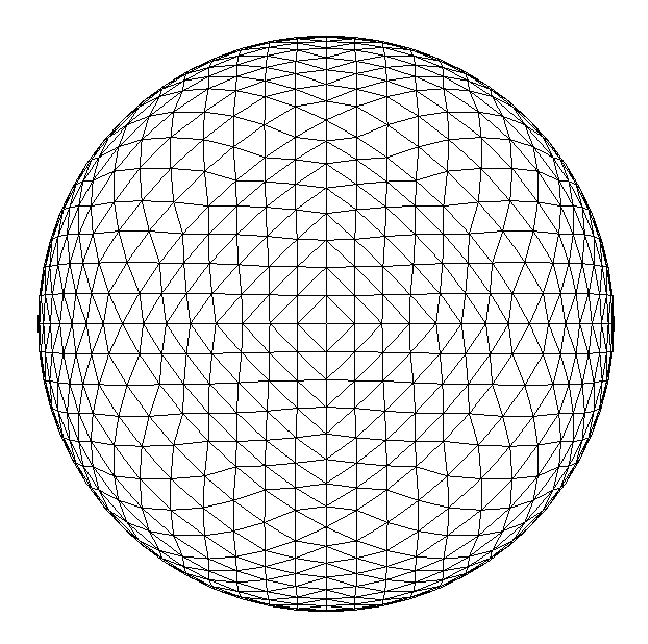
\epsfig{file=heche4octa.ps,height=5.4cm}
\caption{Dual 4-chamfered cube $\Diamond^*_{2048}$}\label{heche3octa}
\end{center}
\begin{center}
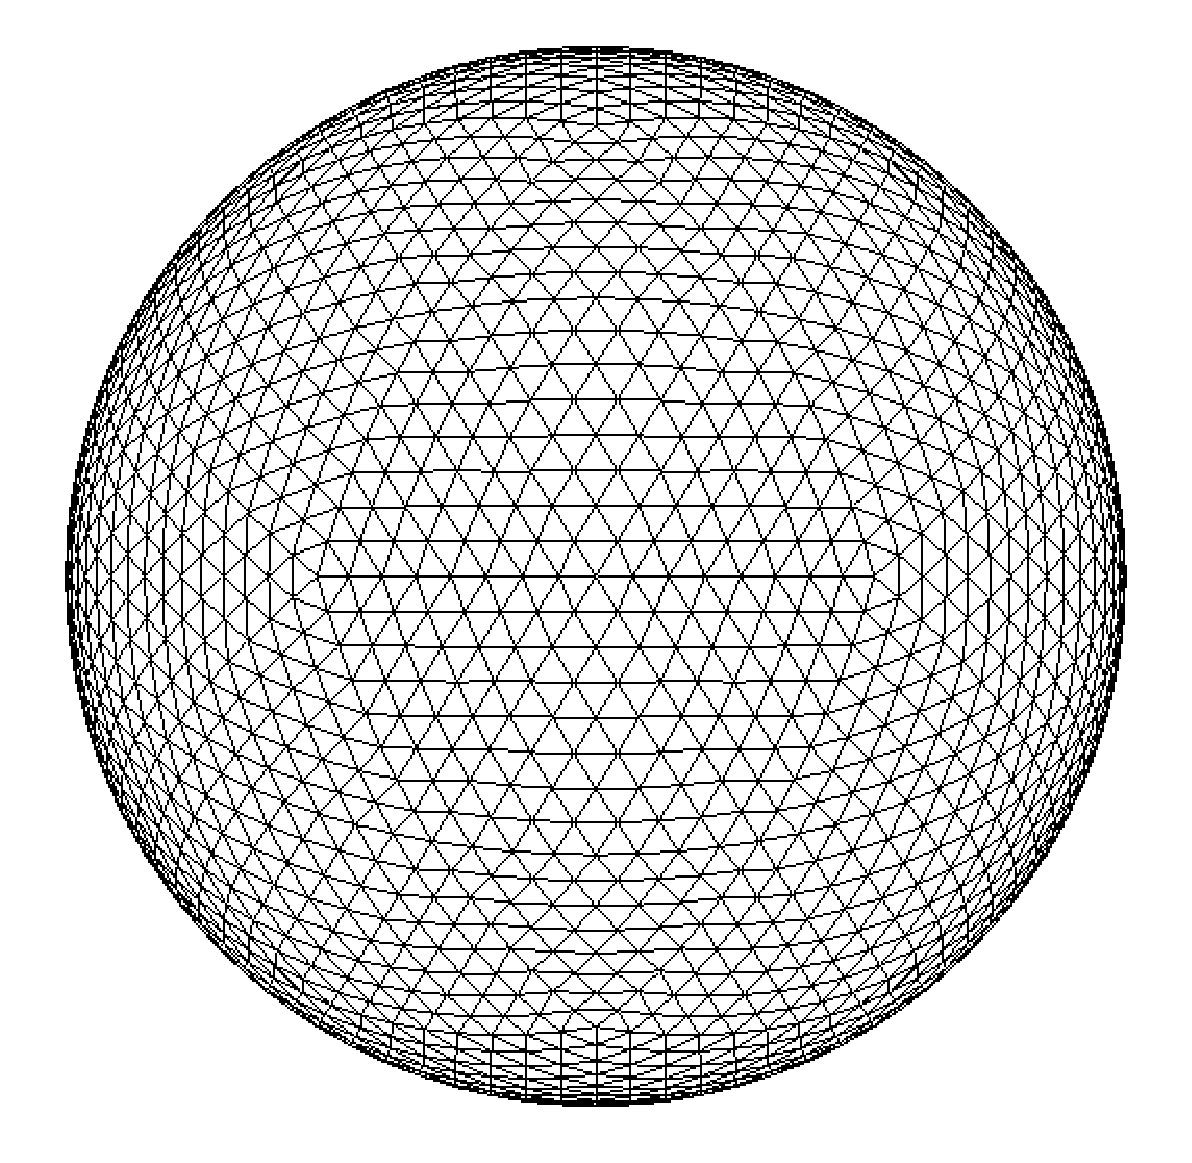
\epsfig{file=heche4dode.ps,height=7.4cm}
\caption{Dual 4-chamfered dodecahedron $C_{5120}^*(I_h)$}\label{heche4dode}

({\it Test planetarium, Iena 1922})
\end{center}
\end{figure}

\newpage
\subsection{Onion-like metallic clusters}\label{cluster}
\subsubsection{Icosahedral and cuboctahedral metallic clusters}
Besides virus capsids and geodesic domes,
the dual $(a,0)$-dodecahedra also occur as levels (concentric {\it onion skins})
in some large metallic clusters (see {\sc Gubin} \cite{gubin} p. 241).
Those {\it $\gamma$-clusters} are made up of $\gamma$ successive shells of atoms surrounding
a central atom, each shell being either a dual $(a,0)$-dodecahedron or a dual $(a,0)$-rhombic 
dodecahedron.
Since an icosahedral shell $C^*_{20a^2}(I_h)$ or a cuboctahedral shell $RhomDode^*_{20a^2}(O_h)$ 
have $10a^2+2$ atoms, the $\gamma$-cluster contains
$1+\sum_{a=1}^{a=\gamma}(10a^2+2)=\frac{(2\gamma+1)}{3}(5\gamma^2+5\gamma+3)$
atoms.
For example, the $561$ palladium atoms of $Pd_{561} L_{60}(OAc)_{180}$
where conjectured in 1985 to realize the icosahedral $5$-cluster; it was proved in 1996 by
{\sc Vagraftik} \cite{vag96} (see Fig. \ref{russia}, taken, with kind permission, 
from \cite{gubin}).
While the $1,2,4$ and $5$-clusters are realized (see Fig. \ref{russia2}) a metallic $3$-cluster
realization is, we believe, not known yet.

\begin{figure}[htbp]
\begin{center}
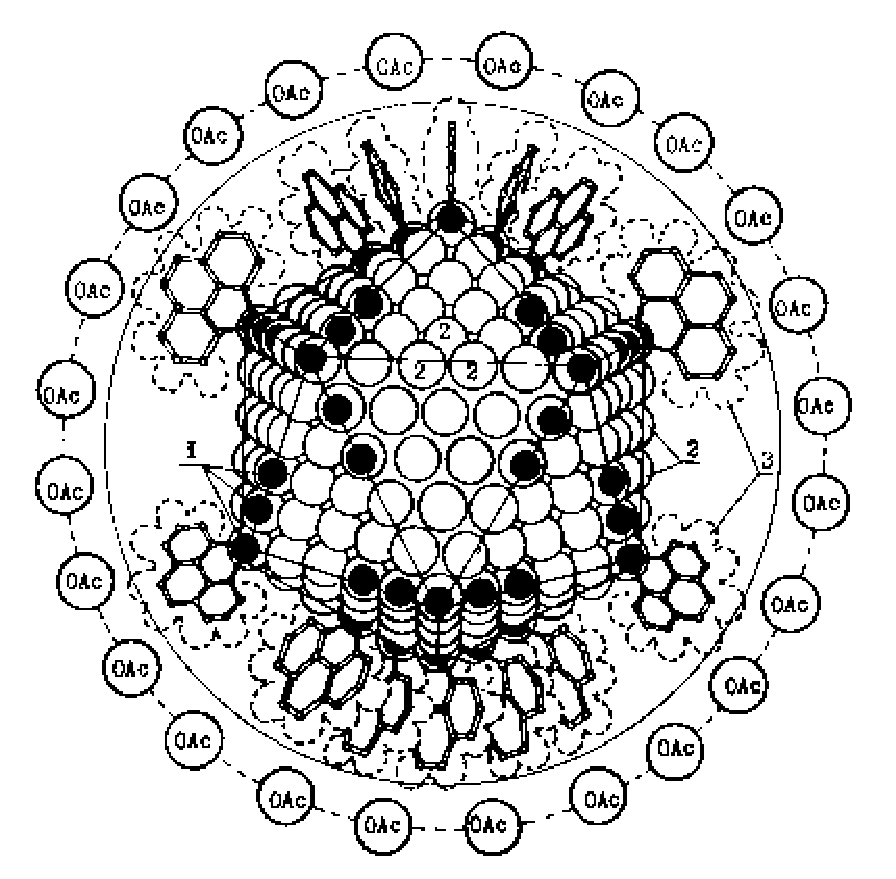
\epsfig{file=russia.ps,width=8.0cm}
\caption{Palladium icosahedral $5$-cluster $Pd_{561} L_{60}(OAc)_{180}$}\label{russia}
\end{center}

\vspace{3mm}
\begin{center}
\begin{tabular}{|c|c|c|c|} \hline
$\gamma$ & Outer shell & Total $\#$ of atoms & Metallic cluster \\ \hline \hline
%$(1,0)$ & $C^*_{20}(I_h)$  &  13  & $[Rh_{13}H_3(Co)_{24}]^{2-}$ \\  \hline
$1$ & $C^*_{20}(I_h)$  &  13  & $[Au_{13}(PMe_2Ph)_{10}Cl_2]^{3+}$ \\  \hline
$2$ & $RhomDode^*_{80}(O_h)$  &  55  & $Au_{55}(PPh_3)_{12}Cl_6$ \\  \hline
%$3$ & $C^*_{180}$ & 147 &  \\  \hline
$4$ & $RhomDode^*_{320}(O_h)$ & 309 & $Pt_{309}(Phen_{36}O_{30\pm 10})$ \\ \hline
$5$ & $C^*_{500}(I_h)$ & 561 & $Pd_{561} L_{60}(OAc)_{180}$ \\  \hline
\end{tabular}
\caption{Icosahedral and cuboctahedral metallic clusters}\label{russia2}
\end{center}
\end{figure}

The evidence for $\gamma$-clusters was also observed as maxima for concentration
profiles of cluster spectra in inert gas, and called there {\it Mackay icosahedra}.
See \cite{esr81} for xenon $3,4$ and $5$-clusters and see \cite{fb83} for
argon $3,4,5$ and $6$-clusters.

\newpage
\subsubsection{Other metallic clusters}
Metallic clusters can also be realized by tetrahedral, octahedral or cubic shells
(see for example \cite{ts85}). The first $5$ metallic clusters given in Fig. \ref{russia4}
are made of only one shell. The last one is made of $2$ non-consecutive octahedral
shells: the dual $(1,0)$ and $(3,0)$-cubes $\Diamond^*_{8}$ and $\Diamond^*_{72}$.
Contrary to the icosahedral and cuboctahedral clusters given in
Fig. \ref{russia2}, those $6$ metallic clusters do not contain a central atom.

\begin{figure}[htbp]
\begin{center}
\begin{tabular}{|c|c|c|c|} \hline
$\gamma$ & Outer shell & Total $\#$ of atoms & Metallic cluster \\ \hline \hline
$1$ & $\triangle^*_{4}$  &  4 & $[H_2Os_4(CO)_{12}]^{2-}$ \\  \hline
$2$ & $\triangle^*_{16}$ & 10 & $[Os_{10}C(CO)_{24}]^{2-}$ \\  \hline \hline
$3$ & $\triangle^*_{36}$ & 20 & $[Os_{20}(CO)_{40}]^{2-}$ \\  \hline \hline
$1$ & $\Diamond_{8}$  &  8  & $[Ni_8(PPh)_6(CO)_8$ \\  \hline \hline
$1$ & $\Diamond^*_{8}$  &  6  & $Rh_6(CO)_{16}$ \\  \hline
$3$ & $\Diamond^*_{72}$ & 44 & $[Ni_{38}Pt_6(CO)_{48}H]^{5-}$ \\  \hline
\end{tabular}
\caption{Some metallic clusters}\label{russia4}
\end{center}
\begin{center}
\epsfig{file=tetra.ps,width=4.0cm}
\caption{Realization of the cluster $[Os_{20}(CO)_{40}]^{2-}$ as dual $(3,0)$-tetrahedron}
\end{center}
\end{figure}

\begin{remark} {\em{\sc (Mackay~\cite{mck})}}
For $\gamma\to\infty$, the infinite onion with outer shell $C^*_{20\gamma^2}(I_h)$
seen as packing of the space by equal spheres is a non-periodic radiating structure
with a unique center. The density of this icosahedral close packing is about
$0.68818$. Replacing the dodecahedron by the rhombic dodecahedron, we get the
face-centered cubic lattice $A_3$ with (maximal among lattices) density of about $0.7405$.
\end{remark}

\newpage
\section{A complete list of embeddable fullerenes?}\label{katsura}
\subsection{ Katsura model for vesicles cells versus embeddable dual fullerenes}
All known fullerenes in which the dual is $\ell_1$-embeddable - including the 
Voronoi plane partition of hexagonal lattice
$A_2$, which can be seen as $C_{\infty}$ - fit the {\sc Katsura} model for coated vesicles cells
(see \cite{k83}). More precisely, the $n$ vertices of a fullerene $F_n$ are partitioned into
$4$ types $T_{a,b}$ according to the number $a$ of pentagons and $b$ of hexagons 
they are incident to, that is, $T_{3,0}$, $T_{0,3}$, $T_{1,2}$ and $T_{2,1}$.
{\sc Katsura} then considers the average strain energy of its $n$ vertices 
assuming Hookean elasticity and only short range interactions.  
The stable fullerenes, that is,  with minimal energy under his model
(depending on which type of vertices have minimal energy)
are the following:

\begin{itemize}
\item[ ]
The dodecahedron (minimal energy on $T_{3,0}$ vertices);
its dual $F^*_{20}(I_h)\rightarrow\frac{1}{2}H_{6}$.

\item[ ]
The hexagonal sheet $C_{\infty}$ (minimal energy on $T_{0,3}$ vertices);
its dual partition $A_2\rightarrow\frac{1}{2}Z\hspace{-2.5mm}Z_{3}$.

\item[ ]
The buckminsterfullerene (minimal energy on $T_{1,2}$ vertices);
its dual $C^*_{60}(I_h)\rightarrow\frac{1}{2}H_{10}$.

\item[ ] 
The elongated hexagonal barrel $F_{36}(D_{6h})$
(minimal energy on $T_{2,1}$ vertices);
its dual $F^*_{36}(D_{6h})\rightarrow\frac{1}{2}H_{8}$.

\item[ ] 
The hexakis truncated tetrahedron $F_{28}(T_d)$
(minimal energy on $T_{2,1}$ vertices);
its dual $F^*_{28}(T_d)\rightarrow\frac{1}{2}H_{7}$.
\end{itemize}
The two other stable fullerenes (with same energy as $F_{36}(D_{6h})$ 
and $F_{28}(T_d)$ and corresponding also minimal energy on $T_{2,1}$ vertices)
are the {\it tennis ball} $F_{32}(D_{3})$ and 
$F_{36}(D_{2d})$ whose duals are not embeddable.\\

Besides fitting the Katsura model, the $C_{60}(I_h)$ is a {\it uniquely elegant structure}
- term %of {\sc Kroto} also 
used by the Nobel committee awarding to {\sc Curl}, {\sc Kroto} and
{\sc Smalley} the 1996 Nobel prize in chemistry for the discovery of the first
fullerene: $C_{60}(I_h)$.
% Its dual, the pentakis dodecahedron, corresponds to the starred (convex-concave)
% dodecahedron, see {\em Gravitation} of {\sc Escher} given in Fig. \ref{escher}.
% The systems of patched $C^*_{60}(I_h)$ is also widely used in architecture.

\subsection{All embeddable fullerenes are known?}
Embeddable fullerenes seem to be extremely rare; we believe that $\{F_{20}(I_h),F^*_{20}(I_h)\}$ 
could be the unique pair of dual $\ell_1$-fullerenes. More precisely, with {\sc M. Shtogrin}, we 
conjecture that all embeddable fullerenes are known, that is: 

\begin{conjecture}$\:$
\begin{itemize}
\item[$(i)$] All $\ell_1$-embeddable fullerenes are: 
$F_{20}(I_h)$, $F_{26}(D_{3h})$, $F_{44}(T)$ and $C_{80}(I_h)$.
\item[$(ii)$] All $\ell_1$-embeddable dual fullerenes are: 
$F^*_{20}(I_h)$, $F^*_{28}(T_d)$, $F^*_{36}(D_{6h})$ and $C^*_{60}(I_h)$.\\
\end{itemize}

\end{conjecture}



\noindent
{\bf Acknowledgments}.
The authors would like to thank 
{\sc 
Gunnar Brinkmann,
Victor Chepoi, 
Alain Dublanchet,
Patrick Fowler,
Branko Gr\"unbaum,
Bruce King,
Thomas Liebling,
Dimitrii Pasechnik,
Andr\'e Rassat} and 
%Mikha\"{\i}l Shtogrin} 
{\sc Tibor Tarnai} for 
pointing out further references, computational help,
advice and encouragements. 
%We wish also to thanks M. C. Escher Heirs and Scientific
%American for their kind permission of reproducing
%of Fig. \ref{escher} and \ref{aids}.

\begin{thebibliography}{99}

\bibitem{a80}
Avis D.:
Hypermetric spaces and the Hamming Cone.
Canadian Journal of Mathematics {\bf 33} (1981) 795-802
\vspace{-3mm}

\bibitem{ad91}
Avis D. and Deza M.:
The cut cone, $\ell_1$-embeddability, complexity and multicommodity flows.
Networks {\bf 21} (1991) 595-617
\vspace{-3mm}

\bibitem{bala95}
Balaban A. T., Liu X., Klein D. J., Babic D., Schmalz T. G., Seitz W. A. and Randic M.: 
Graph invariants for fullerenes. 
Journal of Chem. Inf. Comput. Sci. {\bf 35} (1995) 396-404 
\vspace{-3mm}

\bibitem{b71} 
Berman M.:
Regular faced convex polyhedra. 
Journal of the Franklin Institute, {\bf 291-5} (1971) 329-352
\vspace{-3mm}

\bibitem{brdr}
Brinkmann G. and Dress A.:
A constructive enumeration of fullerenes.
Journal of Algorithms (1997) ({\em to appear})
\vspace{-3mm}

\bibitem{bl77}
Brown L. D. and Lipscomb W. N.:
Closo boron hybrides with 13 to 24 boron atoms.
Organic Chemistry {\bf 16} (1977) 2989-2995
\vspace{-3mm}

\bibitem{ck62}
Caspar D. L. D. and Klug A.:
Physical principles in the construction of regular viruses. 
Cold Spring Harbor Symp. Quant. Biol. {\bf 27} 1-24
\vspace{-3mm}

\bibitem{c71}
Coxeter H. S. M.:
Virus macromolecules and geodesic domes.
In: A spectrum of mathematics
J. C. Butcher ed. Auckland University Press (1971)
\vspace{-3mm}

\bibitem{cdg96}
Chepoi V., Deza M. and Grishukhin V. P.:
A clin d'oeil on $\ell_1$-embeddable planar graphs.
Discrete Applied Math. (1997) 
\vspace{-3mm}

\bibitem{ddmp93} 
Delgado O., Dress A., Muller A. and Pope M. T.: 
Polyoxometalates:A class of compounds with remarkable topology. 
Molecular Engineering {\bf 3} (1993) 9-28 
\vspace{-3mm}

\bibitem{ddub}
Deza A. and Dublanchet A.:
On structure of icosahedral viruses.
({\it in preparation}) 
\vspace{-3mm}
 
\bibitem{dg93} 
Deza M. and Grishukhin V. P.: 
Hypermetric graphs. 
Quarterly Journal of Mathematics Oxford (2) {\bf 44} (1993) 399-433   
\vspace{-3mm}

\bibitem{dg96} 
Deza M. and Grishukhin V. P.: 
A zoo of $\ell_1$-embeddable polytopal graphs.
Bull. Inst. Math. Acad. Sinica (1997)
\vspace{-3mm}

\bibitem{dl94} 
Deza M. and Laurent M.: 
$\ell_1$-rigid graphs.
Journal of Algebraic Combinatorics {\bf 3} (1994) 153-175
\vspace{-3mm}

\bibitem{dl96}
Deza M. and Laurent M.:
Geometry of cuts and metrics.
Algorithms and Combinatorics {\bf 15} Springer-Verlag, Berlin
(1997)
\vspace{-3mm}

\bibitem{ds96} 
Deza M. and Shpectorov S.: 
Recognition of $l_{1}$-graphs with complexity $O(nm)$, or 
Football in a Hypercube.
European Journal of Combinatorics {\bf 17-2,3} (1996) 279-289
\vspace{-3mm}
  
\bibitem{ds00} 
Deza M. and Shtogrin M.:
Isometric embedding of semi-regular polyhedra,
partitions and
their duals into cubic lattices and hypercubes.
Russian Math.Surveys
{\bf 51-6} (1996) 1193-1194
%Uspekhi Mathematicheskikh Nauk 
%{\bf 51-6} (1996) 199-200 ({\it in Russian})
\vspace{-3mm}

%\bibitem{ds98}
%\vspace{-3mm}
%Deza M. and Shtogrin M.:
%Embedding of chemical graphs into hypercubes.
%({\it submitted}), ({\it in Russian}
%\vspace{-3mm}

%\bibitem{dt96} 
%Deza M. and Tuma J.:
%A note on $l_{1}$-rigid planar graphs. 
%European Journal of Combinatorics 
%{\bf 17-2,3} (1996) 157-160
%\vspace{-3mm}

\bibitem{dill}
Dillencourt M. B.:
personal communication (1996)
\vspace{-3mm}

\bibitem{d73}
Djokovi\'c D. \u{Z}.:
Distance preserving subgraphs of hypercubes.
Journal of Combinatorial Theory Series B {\bf 14} (1973) 263-267 
\vspace{-3mm}

\bibitem{ddres}
Dress A., Huson D., and Moulton V..
Analyzing and visualizing sequence and distance data using
SPLITSTREE.
Discrete Applied Mathematics {\bf 71} (1996) 95-109
\vspace{-3mm}

\bibitem{eber91}
Eberhard V.:
Zur morphologie der polyeder. 
Leipzig (1891)
({\it in German})
\vspace{-3mm}

\bibitem{esr81}
Echt O., Sattler K. and Recknagel E.:
Magic numbers for sphere packings: experimental verification in free xenon cluster.
Physical Reviews Letters {\bf 47-16} (1981) 1121-1124
\vspace{-3mm}

\bibitem{e92}
Edmundson J. R.:
The distrubution of point charges on the surface of a sphere.
Acta Crystallographica {\bf A 48} (1992) 60-69 
\vspace{-3mm}

\bibitem{e95}
Elk B. S.:
A canonical assignment of locant numbers to fisular compounds - especially
fullerenes - based on graph theoretical principles.
Journal of Chem. Inf. Comput. Sci. {\bf 35} (1995) 152-158 
\vspace{-3mm}

\bibitem{f86} 
Fleck G.:
Form, Function, and Functioning.
In: Shaping Space. A polyhedral approach. 
M. Senechal and G. Fleck eds.,
Birkh\a"auser, Boston (1986) 151-171
\vspace{-3mm}

\bibitem{flo93}
Florian A.:
Extremum problems for convex discs and polyhedra.
Handbook of Convex Geometry. P. M. Gruber and J. M. Wills eds. 
Elsevier Science (1993) 177-221
\vspace{-3mm}

\bibitem{fow87}
Fowler P. W., Cremona J. E. and Steer J. I.:
Systematics of bonding in non-icosahedral carbon clusters.
Theor. Chim. Acta {\bf 73} (1987) 1-26
\vspace{-3mm}

\bibitem{atlas}
Fowler P. W. and Manolopoulos D. E.:
An atlas of fullerenes.
Clarendon Press, Oxford (1995)
\vspace{-3mm}

\bibitem{fowpi}
Fowler P. W. and Pisanski T.:
Leapfrog transformation and polyhedra of Clar type.
Journal of Chem. Soc. Faraday Trans. {\bf 90} (1994) 2865-2871
\vspace{-3mm}

\bibitem{fk58}
Frank F. C. and Kasper J. S.:
Complex allow structures regarded as sphere packings 1. 
Definitions and basic principle.
Acta Crystallographica {\bf 11} (1958) 184-190
\vspace{-3mm}

\bibitem{fb83}
Friedman J. and Beuhler R. J.:
Magic numbers for argon and nitrogen cluster ions.
Journal of Chemical Physics {\bf 78} (1983) 4669-4673 
\vspace{-3mm}

\bibitem{gasson}
Gasson P. C.:
Geometry of spatial forms.
Ellis Horwood Limited, Chichester (1983)
\vspace{-3mm}

\bibitem{ge92}
G\'evay G.:
Icosahedral morphology.
In: Fivefold Symmetry. I. Hargittai ed. World Scientific,
Singapore - New Jersey - London - Hong Kong (1992) 177-203
\vspace{-3mm}

\bibitem{g35}
Goldberg M.:
The isoperimetric problem for polyhedra.
Tohoku Math. Journal {\bf 40} (1935) 226-236
\vspace{-3mm}

\bibitem{g37} 
Goldberg M.:
A class of multi-symmetric polyhedra.
Tohoku Math. Journal {\bf 43} (1937) 104-108
\vspace{-3mm}

\bibitem{grace}
Grace D. W.:
Search for largest polyhedra.
Mathematics of Computation {\bf 17} (1963) 197-199
\vspace{-3mm}

\bibitem{grun}
Gr\"unbaum B.:
Convex polytopes.
Pure and Appl. Math. {\bf 16} Wiley-Interscience, New York (1967)
\vspace{-3mm}

\bibitem{gubin}
Gubin S. P.:
Khimiya klusterof.
Nauka, Moscow (1987) ({\it in Russian})
\vspace{-3mm}

\bibitem{sloan}
Hardin R. H. and Sloane N. J. A.:
McLaren's improved snub cube and other new spherical designs in three
dimensions.
Discrete Comput. Geom. {\bf 15} (1996) 429-441
\vspace{-3mm}

\bibitem{heppes}
Heppes A.:
Isogonal sph\"arischen netze.
Ann. Univ. Sci. Budapest E\"otv\"os
Sect. Math. {\bf 7} (1964) 41-48 
\vspace{-3mm}
 
\bibitem{chin}
Huang F. Q. and Tang A. C.:
H\"uckel treatment of $B_{32}$ and $B_{92}$.
Journal of Molecular Structure  {\bf 366} (1966) 241-248
\vspace{-3mm}

\bibitem{k85}
Karzanov A. V.:
Metrics and undirected cuts.
Math. Programming {\bf 32} (1985) 183-198
\vspace{-3mm}

\bibitem{k83}
Katsura I.:
Theory on the structure and stability of coated vesicles.
Journal of Theoritical Biology {\bf 103} (1983) 63-75
\vspace{-3mm}

\bibitem{kepler}
Kepler  J.:
Harmonice Mundi (1619)
\vspace{-3mm}

\bibitem{king}
King R. B.:
Topological aspects of chemically significant polyhedra.
Journal of Math. Chemistry {\bf 7} (1991) 51-68
\vspace{-3mm}

\bibitem{kirk}
Kirkman T. P.:
Liverpool Proc. Lit. Philos. Soc. {\bf 37} (1882) 65
\vspace{-3mm}

\bibitem{ks97}
Kuijlaar A. B. J.  and Saff E. B.:
Distrubuting many points on a sphere.
The Mathematical Intelligencer 
{\bf 19-1} (1997) 5-11
\vspace{-3mm}


\bibitem{lhu}
Lhuilier S.:
De relatione mutua capacitatis et terminorum figuranum, etc.
Varsaviae (1782)
\vspace{-3mm}

\bibitem{loeb}
Loeb A.:
Space structures: their harmony and counterpoint.
Addison-Wesley (1976)
\vspace{-3mm}

\bibitem{mck}
Mackay A. L.:
A dense non-crystallografic packing of equal spheres.
Acta Crystallographica {\bf 15} (1962) 916-918
\vspace{-3mm}

\bibitem{mal}
Malkevitch  J.:
Properties of planar graphs with uniform vertex and face structure.
PhD thesis, University of Wisconsin-Madison (1969)
\vspace{-3mm}

\bibitem{m92}
Miyazaki K.:
A mystic  history of fivefold symmetry in Japan.
In: Fivefold Symmetry. I. Hargittai ed. World Scientific
Singapore - New Jersey - London - Hong Kong (1992) 361-393
\vspace{-3mm}

\bibitem{ms90b}
Mosseri R. and Sadoc J. F.:
Geodesic hyperdomes and sphere packing.
International Journal of Space Structures {\bf 5, 3-4} (1990) 325-329
\vspace{-3mm}

\bibitem{dima}
Pasechnik D.:
personal communication (1996)
\vspace{-3mm}

%\bibitem{pc87}
%Pearse B. M. and Crowther R. A.:
%Structure and assembly of coated vesicles.
%Ann. Rev. Biophys. Biophys. Chem. {\bf 16} (1987) 49-68
%\vspace{-3mm}

\bibitem{ppg96}
Plestenjak B., Pisanski T. and Graovac A.:
The minimal non-fullerene Voronoi polyhedra.
Match {\bf 33} (1996) 157-168
\vspace{-3mm}

\bibitem{p54}
P\'olya G.:
Induction and analogy in mathematics.
Princeton University Press, Princeton (1954)
\vspace{-3mm}

\bibitem{msbook}
Sadoc J. F. and Mosseri R.:
Frustration g\'eom\'etrique.
{\em Al\'ea-Saclay}, Eyrolles, Paris (1997) ({\it in French})
\vspace{-3mm}

\bibitem{s94}
Sah C. H.:
A generalized leapfrog for fullerene structures.
Fullerenes Sci. and Tech. {\bf 2 (4)} (1994) 445-458
\vspace{-3mm}

\bibitem{pgr}
Schonland D. S.:
Molecular symmetry - an introduction to group theory and its use in
chemistry.
Gauthier Villars, Paris (1971) 
\vspace{-3mm}

\bibitem{ss94}
Schr\"oder P. and Sweldens W.:
Spherical wavelets: efficiently representing functions on the sphere.
Computer Graphics Proceedings SIGGRAPH 95, ACM Siggraph  (1995)
161-172
\vspace{-3mm}

\bibitem{ss94bis}
Schr\"oder P. and Sweldens W.:
Spherical wavelets: texture processing.
In Rendering Techniques '95.  P. Hanrahan and W. Purgathofer eds. Springer Verlag,
Wien, New York
(1995) 252-263
\vspace{-3mm}

\bibitem{s93}
Shpectorov S.: 
On scale-isometric embeddings of graphs into hypercubes. 
European Journal of Combinatorics {\bf 14} (1993) 117-130 
\vspace{-3mm}

%\bibitem{sloan2}
%Sloane N. J. A., Hardin R. H., Duff T. D. S. and Conway J. H.:
%Minimal-energy clusters of hard spheres.
%Discrete and Computational Geometry {\bf 14} (1995) 237-259
%\vspace{-3mm}

\bibitem{stein}
Steiner J.:
Sur le maximum et le minimum des figures.
J. Math. Berlin {\bf 24} (1842) 93-152 and 189-250
\vspace{-3mm}

\bibitem{tarnai} 
Tarnai T.:
Geodesic domes: natural and man-made.
International Journal of Space Structures {\bf 11, 1-2} (1996) 
\vspace{-3mm}

\bibitem{tarnai2}
Tarnai T.:
Geodesic domes and fullerenes.
Phil. Trans. R. Soc. London {\bf A 343} (1993) 145-154
\vspace{-3mm}

\bibitem{ts85}
Theo B. K. and Sloane N. J. A.:
Magic numbers in polygonal and polyhedral clusters.
Inorganic Chemistry {\bf 24} (1985) 4545-4558
\vspace{-3mm}

\bibitem{thim}
Thimmappa B. H. S.:
Low valent metal clusters - an overview.
Coord. Chem. Reviews {\bf 143} (1995) 1-34
\vspace{-3mm}

\bibitem{uk92}
Ulick\'y L. and Kemp T. J.:
Comprehensive dictionary of physical chemistry. 
PTR Prentice Hall (1992)
\vspace{-3mm}

\bibitem{vag96}
Vagraftik M. N.:
Gigantic clusters of palladium.
Coordination Chemistry {\bf 22-5} (1996) 352-357 ({\it in Russian})
\vspace{-3mm}

\bibitem{w84} 
Wells A. W.: 
Structural Inorganic Chemistry. IV ed.
Oxford (1984) 
\vspace{-3mm}

\bibitem{Za}
Zalgaller V. A.: 
Convex polyhedra with regular faces.  
Seminar in Mathematics of V. A. Steklov Math. Institute, Leningrad {\bf 2}
Consultants Bureau, New York (1969)  
\vspace{-3mm}

\end{thebibliography} 


\vspace{5mm}
\noindent
{\small Antoine DEZA}\\
{\em Ecole Polytechnique F\a'ed\a'erale de Lausanne, d\a'epartement de
math\a'ematiques, CH-1015 Lausanne, Suisse. 
Email:  deza{\small @}masg1.epfl.ch}\\
and\\
{\em Ecole des Hautes Etudes en Sciences Sociales, 
centre d'analyse et de math\a'ematique sociales, 54 Bld Raspail, Paris, 
France.
Email:  deza{\small @}ehess.fr}\\\\
{\small Michel DEZA}\\
{\em CNRS, Ecole Normale Sup\a'erieure, d\'epartement
de math\'ematiques et informatique, 45 rue d'Ulm, Paris, France.
E-mail: deza{\small @}dmi.ens.fr}\\\\
{\small Viatcheslav GRISHUKHIN}\\
{\em CEMI, Russian Academy of Sciences, Krasikova 32, Moscow 117 418, Russia.
E-mail:\linebreak grishuhn{\small @}serv2.cemi.rssi.ru}

%\newpage
\listoffigures

\end{document}
